\documentclass[]{svjour3}
\RequirePackage{fix-cm}
\usepackage[utf8]{inputenc}
\usepackage[usenames,dvipsnames]{color}
\usepackage{fullpage}

\usepackage[numbers, sort, compress]{natbib}
\usepackage{graphics}
\usepackage{graphicx}
\usepackage{epstopdf}
\usepackage{color}
\usepackage{hyperref}
%\usepackage{pdfsync}
\usepackage{mdwlist}
\usepackage{colortbl}

\begin{document}

\title{Distributed Application Runtime Environment (DARE): A
  Standards-based Framework For Developing Science Gateways}

\author{Joohyun Kim \and Sharath Maddineni \and Yaakoub El-Khamra \and
  Shantenu Jha}

\institute{Center for Computation and Technology, Louisiana State
  University, \email{jhkim@cct.lsu.edu} \and Center for Computation
  and Technology, Louisiana State University,
  \email{smaddineni@cct.lsu.edu} \and Center for Computation and
  Technology, Louisiana State
  University, % Bioinformatics Laboratory, Academic Medical Center, University of Amsterdam, \email{m.a.santcroos@amc.uva.nl}
  \and Texas Advanced Computing Center, TACC, The University of Texas
  At Austin, \email{yaakoub@tacc.utexas.edu} \and Center for
  Computation and Technology, Louisiana State University, Rutgers
  University, School of Informatics, University of Edinburgh,
  Department of Computer Science, Louisiana State University,
  \email{shantenu.jha@rutgers.edu}}

%\titlerunning{Dynamic Application Runtime Environment (DARE): A Standards-based Framework For Science Gateways}
%\authorrunning{Joohyun Kim et al.}

%\keywords{Science Gateways}
%\subclass{ MSC codes }
%\PACS{ PACS codes }
%\CRclass{ CR codes }

\date{Received: date / Accepted: date}


% \begin{center}
%   Joohyun Kim$^{1}$, Sharath Maddineni$^{1}$, Mark Santcroos$^{1,4}$,
%   Yaakoub El-Khamra$^3$, Shantenu Jha$^{1,2,5,6}$\\
%   $^1$ Center for Computation and Technology, Louisiana State University\\
%   $^2$ Rutgers University
%   $^3$ Texas Advanced Computing Center, TACC, The University of Texas At Austin \\
%   $^4$ Bioinformatics Laboratory, Academic Medical Center, University of Amsterdam\\
%   $^5$ School of Informatics, University of Edinburgh\\
%   $^6$ Department of Computer Science, Louisiana State University\\
% \end{center}


%\numberofauthors{3}
% \author{
% \alignauthor Joohyun Kim\\
%        \affaddr{Center for Computation and Technology}\\
%        \affaddr{Louisiana State University}\\
%        \affaddr{216 Johnston}\\
%        \affaddr{Baton Rouge, LA} \\
%        \email{jhkim@cct.lsu.edu}
% \alignauthor Sharath Maddineni\\
%        \affaddr{Center for Computation and Technology}\\
%        \affaddr{Louisiana State University}\\
%        \affaddr{216 Johnston}\\
%        \affaddr{Baton Rouge, LA}
%        \email{smaddineni@cct.lsu.edu}
% \alignauthor Mark Santcroos\\
%        \affaddr{}\\
%        \affaddr{}\\
%        \affaddr{}\\
%        \affaddr{} \\
%        \email{}
% \alignauthor Yaakoub El-Khamra\\
%        \affaddr{}\\
%        \affaddr{}\\
%        \affaddr{}\\
%        \affaddr{} \\
%        \email{}
% \alignauthor Shantenu Jha 
% \titlenote{Author for correspondence}\\
%       \affaddr{Rutgers University, Piscataway, NJ 08854, US  }\\
%       \affaddr{CCT, Louisiana State University}
% %      \affaddr{214 Johnston}\\
%       \affaddr{Baton Rouge, LA, 70803, US}
%      \email{sjha@cct.lsu.edu}
% }


  % An understanding of challenges and computational requirements of
  % the life-science applications suggests that the uptake of
  % distributed heterogeneous scalable HPC resources demonstrate its
  % effectiveness as an integral component of a wide-range of
  % life-science gateways. DARE science gateways comprise a user
  % access layer and middleware layers built upon Simple API for Grid
  % Application (SAGA) and the SAGA-based Pilot-Job (SAGA-BigJob)
  % capability.
\maketitle

  % However, there are missing capabilities and abstractions that
  % enable the use of the collective capacity of distributed
  % cyberinfrastructure such as TeraGrid/XSEDE, especially those that
  % can be used to develop gateways in an easy, extensible and
  % scalable fashion for both compute and data-intensive applications.

 % However, there are missing capabilities that make distributed
  % cyberinfrastructure such as TeraGrid/XSEDE usable as a
  % collective resource difficult; these missing abstractions include
  % those that can be used to develop Gateways to utilize the
  % collective capacity of distributed cyberinfrastructure in an easy,
  % extensible and scalable fashion for both compute and
  % data-intensive applications.  This is a serious barrier, as
  % Gateways often require customization for specific user groups and
  % infrastructure usage modes.  So whereas a single science gateway
  % is a scalable access mechanism in terms of number of people, that
  % can be supported, the development of multiple similar gateways but
  % with differing infrastructure usage and requirements is not
  % scalable.

% that supports the utilization of distributed resources
%   for both compute and data-intensive applications.


  \begin{abstract}
    Gateways have proven to be a very effective mechanism to utilize
    distributed HPC resources.  Gateways have been able to provide
    efficient and simplified access for the most common requirements
    for ``the masses'', as well as proving successful as a
    shared-community access mode to production cyberinfrastructure
    such as the TG/XSEDE.  However, missing capabilities that make
    using production cyberinfrastructure as a collective resource
    difficult have also been a serious barrier in the utilization of
    the collective capacity of distributed cyberinfrastructure by
    Science Gateways too.  The development of multiple similar
    gateways that can work over a range of production
    cyberinfrastructures, usage modes and application requirements
    %but with differing production cyberinfrastructure usage
    %and requirements 
    is not scalable without a well-designed, effective and extensible
    framework. We introduce the SAGA-based, Distributed Application
    Runtime Environment (DARE) framework, using which gateways that
    seamlessly and effectively utilize scalable distributed
    infrastructure are built. % We analyze a range of life-science
%     applications, and establish that DARE provides a framework which
%     meets the needs of life-science applications, i.e.,
    DARE along with SAGA provides effective interoperable middleware
    upon which to build such gateways.  We discuss the architecture of
    the DARE framework and discuss how gateways can utilize the
    framework. We discuss several initial prototypes -- DARE-HTHP,
    DARE-NGS, of DARE-based gateways for life-science applications.
\end{abstract}

%  This work is predicated on three important trends: (i) that the
%   importance, impact and percentage of TeraGrid/XSEDE resources
%   assigned to the life sciences is increasing at a rate that is
%   probably greater than other disciplines, (ii) that gateways have
%   proven to be a very effective access mechanism to distributed HPC
%   resources provided by the TeraGrid/XSEDE, and in particular a very
%   successful model for shared/community access models, and (iii) that
%   in spite of the previous two points there are missing capabilities
%   and abstractions that enable the use of the collective capacity of
%   distributed cyberinfrastructure such as TeraGrid/XSEDE, especially
%   those that can be used to develop gateways in an easy, extensible
%   and scalable fashion for both compute and data-intensive
%   applications. We introduce the SAGA-based, Dynamic Application
%   Runtime Environment (DARE) framework from which extensible,
%   versatile and effective gateways that seamlessly utilize scalable
%   infrastructure can be built for a life-science applications. We
%   discuss the architecture of DARE-based gateways, and particularly
%   life-science gateways -- DARE-HTHP, DARE-NGS, DARE-RFOLD, and
%   DARE-DOCK, that use the DARE-framework to support a wide-range of
%   life-science capabilities.


\newif\ifdraft
\drafttrue                                                                                        \
\ifdraft
 %\newcommand{\reviewer}[1]{ {\textcolor{blue}    { ***Reviewer:     #1 }}}
 \newcommand{\jkimnote}[1]{{\textcolor{green}   { ***Joohyun:   #1 }}}
 \newcommand{\jhanote}[1]{  {\textcolor{red}     { ***SJ: #1 }}}
  \newcommand{\smnote}[1]{  {\textcolor{red}     { ***Sharath: #1 }}}
 \newcommand{\todo}[1]{  {\textcolor{red}     { ***TODO: #1 }}}
 \newcommand{\fix}[1]{  {\textcolor{red}     { ***FIX: #1 }}}
\newcommand{\yyenote}[1]{  {\textcolor{blue}     { ***YYE: #1 }}}
 \newcommand{\reviewer}[1]{}
\else
 \newcommand{\reviewer}[1]{}
 \newcommand{\yyenote}[1]{}
 \newcommand{\jkimnote}[1]{}
 \newcommand{\smnote}[1]{}
 \newcommand{\jhanote}[1]{}
 \newcommand{\todo}[1]{  {\textcolor{red}     { ***TODO: #1 }}}
 \newcommand{\fix}[1]{}                                                                              
 \fi



% \category{D.1.3}{Software}{Concurrent Programming}{ Distributed programming/parallel programming} 
% \category{J.3}{Computer Applications}{Bioinformatics}

% \section*{General Terms}{Design,Measurement,Theory}

%  \keywords{Science Gateway, Runtime Environment, Distributed Computing, Simple API for Grid
%   Applications (SAGA), Pilot-Job abstraction, Data-intensive Computing}

\section{INTRODUCTION}


% as seen from Figs.~\ref{tg2007} \& \ref{tg2008} and
% Table~\ref{tg2011}, the trends are somewhat unambiguous: among
% consumed computing resources via TeraGrid (TG), now XSEDE, the
% NSF-funded nationwide Cyberinfrastructure (CI) started in 2001 and
% operated between 2004 and 2011 in the USA, the percentage devoted to
% the life sciences is already more than any discipline and the usage
% seems to be increasing, whether measured by number of cycles consumed,
% users or allocations~

% The single largest community is the life-sciences community --
% including MD (25\%)... Get a break-down of the total usage of the TG
% by discipline and application type.

In spite of fundamental limitations on the precision of the data,
amongst the many indicators of the importance of computing in the life
sciences, is the fact that for most production distributed
cyberinfrastructure, the proportion of resources devoted to the life
sciences is already more than any discipline and the usage seems to be
increasing. This is valid whether measured by number of cycles
consumed, users or allocations.  However, this rise has been dominated
by a few well-established domains,
% In other words, the massive
% increase in the proportion of resources utilized by the life-sciences
% is skewed by the dominance of the
such as large-scale Molecular Dynamics (MD) simulations, and
phylogenetics.  The former has benefited from the availability of
multiple community codes, tailored to the effectively utilize the
computing infrastructure, thus enabling easy uptake/usage amongst the
scientific community.  The need for large-scale distributed parallel
execution for other areas of life-science applications is growing.  A
specific example highlighting trends and advances in experimental
techniques producing large scale data sets with their high-throughput
methods, is provided by Next-Generation DNA Sequencing (NGS), and it
associated challenge of increasing computational sophistication
required in the gathering, management, and the analysis of derived and
produced data.

% due to the as well as the advent of computing power and data
% management capacity.

% and consequent challenges arises in the context of Next-Generation DNA
% Sequencing (NGS) technologies, with unprecedented amounts of data
% produced through high-throughput methods and increasing computational
% requirements for gathering, management, and the analysis of associated
% or produced data sets along a pipeline process.

 
% However, most life-science applications have not been very effective
% in utilizing HPC cyberinfrastructure.

% Commented out by yye00, figure is referenced in a paragraph that has been commented out
% \begin{figure}
%  \centering
% 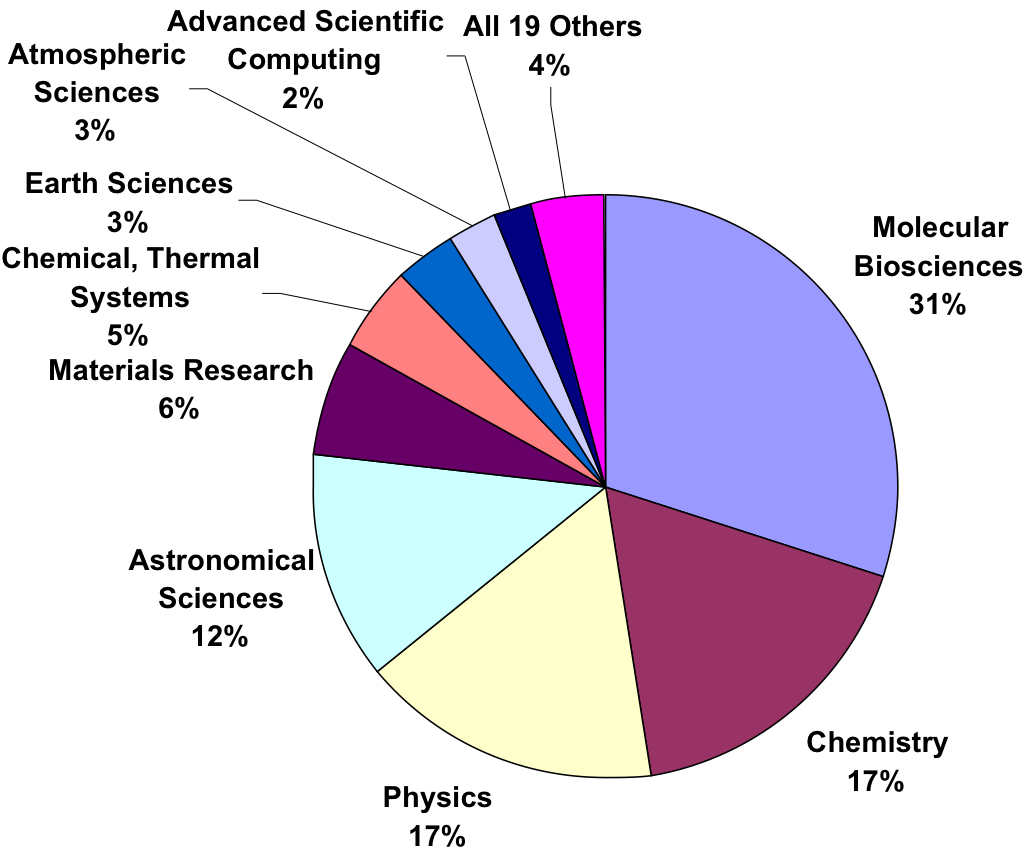
\includegraphics[scale=0.40]{figures/teragrid-discipline07}
% \caption{\small 2007 Usage statistics for the TG. (Reference
%   \url{http://www.teragridforum.org/mediawiki/images/9/90/II_WorkShop_G-HPC_Nework_2009-Towns.pdf})}
%   \label{tg2007}
% \end{figure}


% MD simulations have mostly relied on scaling-up to high core-counts,
% whilst virtual docking calculations benefits from high-throughput
% calculations.  with the exception of a few common applications,
% e.g., large-scale simulations (mostly Molecular Dynamics(MD)) and
% virtual-docking simulations,


% represents a case that

% for analyzing large volumes of data are
% effectively managed.

% required data analytics required
% along with dealing with 

%A specific example highlighting these trends and consequent challenges

On the other hand, Science Gateways have witnessed impressive
achievements in terms of the growth of the number of supporting
researchers and computing time usages~\cite{gce11-nancy}. According to
the very recent report about TG/XSEDE Science Gateway
program~\cite{gce11-nancy}, whereas, in 2006, 10 gateways consumed
100,000 CPU hours, in 2010, 22 gateways provided 40 million hours
usage; by 2011 nearly 40\% of users on TG/XSEDE came through TG/XSEDE
gateways. Interestingly, the CIPRES phylogenetic gateway, which was
notably absent a few years ago, accounts for 25 \% of all TG/XSEDE
users in 2011. Such rapid and broad uptake of gateways, is indicative
of their potential of supporting existing and novel scientific
computing practices and consequently for advancing associated
scientific domains.

%  exceeding other gateways dedicated to
% traditionally large-scale scientific computing domains, indicating a
% great potential of the gateway development for nurturing novel
% scientific computing practices and consequently for advancing
% associated scientific domains.
 
Based on the usage of the TG/XSEDE Science Gateways in first quarter
of 20011, 3-4 of $\approx$ 20 TG/XSEDE gateways currently are
biological/life science, which in turn account for about $\approx$
35\% of all gateway cycles used. Helped by the aforementioned four
gateways, although existing life-science gateways account for a
significant fraction of all gateway cycles usage, access to TG/XSEDE
via gateways accounts for only %2-3\% of
a fraction of all cycles devoted to biosciences
%all cycles used, even though molecular biosciences
(which by most accounts represented 25\% of TG/XSEDE (NU) cycles used
in Q1-2011.~\footnote{It is difficult to provide such information in a
  consistent way as the total number of cycles available year-to-year
  varies, but also which discipline a proposal gets assigned to is
  somewhat random; thus many chemistry proposals, even physics
  proposals are likely to be biological in nature. Also, although we
  are referring to life-science applications in general information is
  provided under bio-molecular bio-sciences which are understood to
  represent a large fraction of computational life-science
  applications.})  Thus although a significant fraction of TG/XSEDE
cycles are devoted to molecular biosciences, of which MD is the
dominant component, only a few of the MD users actually use gateways
to access TG/XSEDE resources.  By most accounts at best only 10\% of
all life-science applications cycles are accessed via gateways.
Additionally, the dominant growth in computing is coming from novel
application areas such as NGS which can benefit from community
provided gateways.

Thus given the overall success and uptake of the gateways approach,
{\it prima facie} there are reasons to believe that if a scalable,
effective and extensible capability were provided for life-science
applications, this {\it gap} could be overcome.



% However, these 4 gateways account
% for about 2-3\% of recording molecular bioscience usage.
%  by some
% accounts representing 25\% of TG/XSEDE~\footnote{It is difficult to
%   provide such information in a consistent way as the total number of
%   cycles available year-to-year varies, but also which discipline a
%   proposal gets assigned to is somewhat random; thus many chemistry
%   proposals, even physics proposals are likely to be biological in
%   nature.}  (NU) cycles used in Q1-2011,

 
% Commented out by yye00, paragraph where this is used has been commented out
% \begin{figure}
%  \centering
% 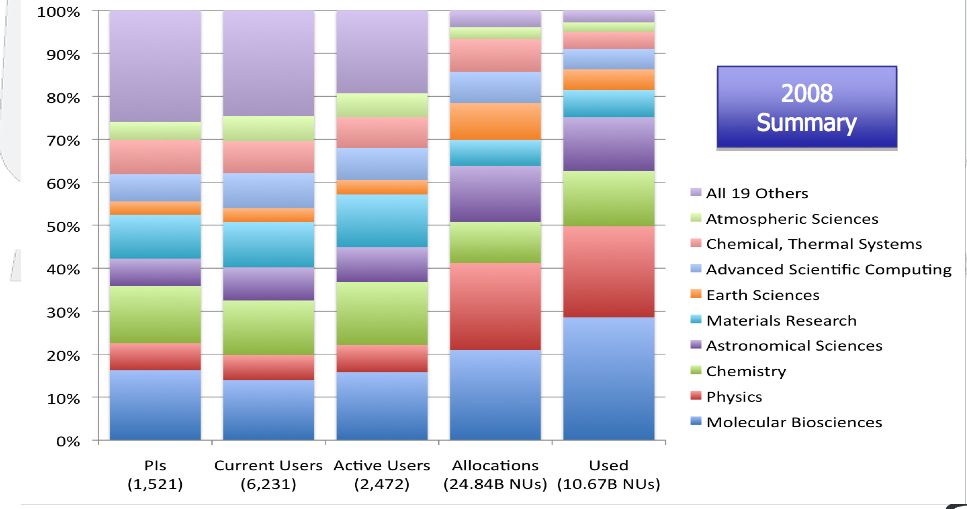
\includegraphics[scale=0.27]{figures/teragrid-discipline08}
% \caption{\small 2008 Usage statistics for the TG/XSEDE (Reference
%   \url{http://www.teragridforum.org/mediawiki/images/d/d8/DEISA-PRACE-May2009-Towns.pdf})}
%   \label{tg2008}
% \end{figure}

Interestingly, the cyberinfrastructure (CI) considerations required to
support a broad-range of analytical approaches and at the scales
required, has received less attention than the data-management problem
and algorithmic advances. Thus not surprisingly, traditional
production cyberinfrastructure, such as the TG/XSEDE, have not been used for
such data-intensive analytics and distributed applications. There are
multiple reasons, but a couple of contributing factors are: (i)
insufficient runtime environments (and abstractions) to support
concurrent computational capabilities with large-data sets to support
data-analytics (beyond visualization) in an easy, scalable and
extensible fashion, (ii) insufficient support for user-customizable
data-intensive "workflows" that effectively hide the challenges of
data-movement and efficient data-management whilst managing concurrent
distributed (computational) resources.

These provide the two primary motivations of our work: the first is
the immense potential and advantage of providing gateways for
life-science applications, and thus a strategic opportunity. The
second is derived from missing capabilities to support existing and
emerging science gateways (e.g., data-intensive applications) to
utilize distributed cyberinfrastructure in a scalable and extensible
fashion.

% {\it Towards a common middleware for Gateways:} A fundamental design
% objective of Science Gateways is to capture the common requirements of
% the science scenarios, make it easy to support their computational
% requirements, whilst providing the right abstractions to support them
% and making the application/usage-mode specific parts easy to support.
% This objective imposes an important constraint and requirement on the
% tools \& frameworks used to develop Science Gateways.

% to enable/facilitate/support them by making the application/usage-mode
% specific parts easy to support.
%it aims to enable and to provide

{\it Towards a common middleware for Gateways:} Building effective science gateways
has two major tracks: the first is the development of an effective UI
and tools that capture application requirements, e.g., expression of
workflows etc, and making these accessible via community/shared
accounts with proper security and credentials supported. These must be
customizable and extensible to the end-user communities need and
specific scientific requirements. The second is the integration of
these UI/tools with a broad range of high-performance and distributed
computational (HPDC) infrastructure to support
the science requirement, but in a way that is scalable and flexible.
These require different types of often non-overlapping tools and
expertise.  A fundamental design objective of Science Gateways is to
capture and support the common requirements of the science scenarios,
and to support them in a simple and extensible fashion by providing
the right abstractions.  This objective imposes
important %constraint and
requirements on the middleware, tools and frameworks used to develop
Science Gateways.

Many gateway developments are often helped by a suite of development
frameworks such as the Open Grid Computing
Environments\cite{ogce-2010} (OGCE); however development frameworks
such as OGCE do not support the integration with the underlying HPDC
infrastructure, i.e., most gateways still enforce the tight-coupling
between applications and a specific infrastructure (see
table~\ref{table:TG-sg}), without support for flexible distributed
execution.  A primary reason is the additional and significant
complexity in %providing the right abstractions so as to enable an
enabling applications to seamlessly utilize distributed
cyberinfrastructure. Such requirements become harder to achieve as the
number of connected sites and heterogeneity grows (interestingly, both
the TG in its transition to eXtreme Science and Engineering Discovery
Environment (XSEDE)~\cite{XSEDE} and EGEE in its transition to EGI
increased the number of middleware distributions they ``support''.
XSEDE supports globus, UNICORE and GENESIS; EGI supports gLite,
Globus, ARC and UNICORE).

% seamlessly transform a target application to be able to seamlessly ,
% and thus into a distributed application.

% as well as the computing power and the data storage capacity of each
% resource reach peta or exa scales.

\begin{table}
\centering
 \small
\begin{tabular}{|c|c|c|c|c|c|} 
  \hline  Quarter & PIs & Current & Active & Allocations  & Usage\\
  & & Users  &  Users & (NUs) $\times 10^6$& (NUs) $\times 10^6$ \\ \hline
  Q3 2010 & 249 & 1,044 & 366 & 8,810   & 2,219  \\ \hline
  Q4 2010 & 254 & 1,040 & 356 & 11,720  & 2,658, \\ \hline
  Q1 2011 & 257 & 1,168 & 418 & 13,101  & 3,412\\ \hline 
\end{tabular} 
\caption{Life-Science usage of the TG/XSEDE over the recent
  quarters. The figures establish that both the  allocation and the
  usage of life-science applications is increasing at least in
  proportion to the increasing resource availability on the TG/XSEDE,
  if not faster.}
 \label{tg2011} 
\end{table}


%\jhanote{Need to discuss}


% which is often eased by the development of a framework.  More
% importantly, supporting a \jhanote{need to define? why should the
%   reader care?}  is critical considering different application usage
% modes for different life-science applications.  \yyenote{The
%   following is a confusing sentence}\jkimnote{I tried to change it}

Viewed from a different perspective, there are hard challenges (i.e.,
integrating with heterogeneous HPDC infrastructure) and there are
application/usage scenario specific challenges in building science gateways. The
contribution of this work is to address the former challenge via the
development of middleware for Gateways so as to support the effective
integration of these two different tracks, viz., enable different
application-specific UIs (and security contexts) to utilize a range of
high-performance and distributed computational (HPDC) infrastructure.

The role of effective middleware is to support maximum reusabilty of
the challenging effort in integrating with HPDC infrastructure.  with
minimal repetition of effort.  For example, it is always challenging
to integrate new applications, to implement distributed data
management with newly added infrastructure, whilst supporting existing
and novel execution patterns; any framework that aims to facilitate
integration with HPDC infrastructure must also address these
challenges.  Thus any framework used to build science gateways that provides simple
and scalable integration with the HPDC infrastructure must support
broad range of diverse execution patterns (i.e., commonly occurring
modes of using HPDC infrastructure).

Specifically, we address the following problem: Although, Science
Gateways have proven to be very effective access mechanism to
distributed HPC resources provided by the production
cyberinfrastructure such as TeraGrid/XSEDE and in particular a very
successful model for shared/community access models, however, there
are missing capabilities and abstractions that enable the use of the
collective capacity of distributed cyberinfrastructure such as
TeraGrid/XSEDE, especially those that can be used to develop a range
of functionally similar yet slight different gateways in an easy,
extensible and scalable fashion for both compute and data-intensive
applications.

% As shown in Table~\ref{table:four-applications},
% flexible execution/usage of four life-science applications are
% summarized by contrasting conventional versus distributed modes.


% \yyenote{The following is the same incredibly long 3 sentences rolled into 1 from the abstract. Needs a bit of change}

% This work is predicated on three important trends: (i) that the
% importance, impact and percentage of TG/XSEDE resources assigned to the
% life sciences is increasing at a rate that is probably greater than
% other disciplines, (ii) that gateways have proven to be a very
% effective access mechanism to distributed HPC resources provided by
% the TG/XSEDE (and in particular a very successful model for
% shared/community access models); given the landscape of the future
% distributed cyberinfrastructure, we anticipate the importance of
% gateways will continue to increase, and (iii) that there are missing
% capabilities and abstractions to enable the use of the collective
% capacity of distributed cyberinfrastructure such as TG/XSEDE, especially
% those that can be used to develop gateways in an easy, extensible and
% scalable fashion for both compute-intensive and data-intensive
% applications.


% gateway development concentrates on the
% development of a runtime environment for distributed applications. T

We introduce the Distributed Application Runtime Environment (DARE)
framework; we illustrate and demonstrate the development of a runtime
environment that supports as a primary design objective the
distributed execution of applications on HPDC infrastructure.  In
general, DARE supports the general goals of distributed applications:
interoperability, dynamic execution %distributed scale-out,
extensibility, adaptivity, scalability (scale-up, scale-out and
scale-across) -- referred to as IDEAS~\cite{ideas}.  DARE builds upon
and utilizes SAGA to achieve the IDEAS objective.  {\it Scale-up} --
or the most common type of scaling behavior, refers to the need of a
single simulations of using many cores efficiently; {\it scale-out} is
a measure of the ability to support the concurrent execution and
management of multiple tasks/jobs respectively (either on a single
resource, or across multiple physically distributed resources); {\it
  Scale-across} is raised by the need to efficiently distribute across
multiple distinct and possibly heterogeneous resources. {\it
  Adaptivity} addresses the requirement that distributed applications
may have to adapt to resource fluctuation across platforms, and to the
availability of dynamic data.

\begin{table}
\centering
 \small
\begin{tabular}{|c|c|c|c|} 
  \hline Gateway  & Science f & Infrastructure & Execution Mode 
  \\
  Name & Domain & Used & \\ 
  &  &  & \\
  & & & \\  \hline \hline 
  
  CIPRES   & phylogeny  &  single node  & multiple  \\
   &  &   & independent   \\ 
  &  &  &  tasks \\  \hline
  GridChem   & quantum & single node or     & multiple  \\
     & chemistry, & small cluster & independent   \\
  & MD &  & task  \\ \hline
   GridAMP     & ASTEC  & legacy domain  & pipelined \\ 
  & coupled with  &  scientific code   & HPC  \\
  & a parallel GE &   &  programs \\ \hline
  Nano  & portal  & large set   & multiple \\
  Hub  & for nano- & of tools  & independent \\
   & technology &  & tasks \\ \hline
  \hline
\end{tabular} \caption{Examples of existing TG/XSEDE Science Gateways. The list is not necessarily complete. More information including URLs can be found elsewhere \cite{tg-sg-list-url}. ASTEC means Aarhus Stellar Evolution Code.}
 \label{table:TG-sg} 
\end{table}

Before we introduce the DARE framework we discuss the ``D'' in
DARE. Although the ``D'' is for Distributed, a fundamental attribute
of many applications -- distributed or otherwise, and infrastructure
that DARE is designed to support is that of ``dynamism''.  Dynamic
aspects come from both an understanding of applications/analytical
requirements as well the runtime/infrastructure characteristics.  The
fact that applications can change as a consequence of the results
produced or the analytical requirements often means that minor changes
in the application (run-time) properties/results often lead to large
differences in the HPDC infrastructural requirements, duration of runs
etc. The HPDC infrastructure utilized often varies, and thus runtime
decisions related to scheduling and resource aggregation need to be made.

%\yyenote{Insert pilot job definition here. Moved reference}

Pilot-jobs provide a simple approach for decoupling workload
management and resource assignment/scheduling, via the concept of
utilizing a placeholder job as a container for a set of compute tasks.
They thus provide an effective abstraction for dynamic execution and
resource utilization in a distributed context.
Pilot-Jobs~\cite{pstar11} have been shown to be an excellent
abstraction for supporting dynamic/runtime resource allocation and
selection.  In fact, there are reasons to expect Pilot-Jobs as an
excellent abstraction to support the formulation of dynamic
applications as well~\cite{pstar11}. Pilot-Jobs are particularly well
suited for distributed environments.  We have shown that a flexible
Pilot-Job framework can provide the ability to run many MD simulations
effectively across multiple resources on the
TG/XSEDE~\cite{saga-royalsoc,saga_bigjob_condor_cloud}.  Specifically,
we've shown how a SAGA-based implementation of the pilot-job, supports
the distributed application design objectives categorized by the term
IDEAS\cite{ideas}.

As we will discuss in the next section, the DARE framework makes
extensive use of Pilot-Jobs and is also designed to support
distributed and dynamic applications as a primary/fundamental
attribute.  In this paper we establish how these capabilities can be
generalized to a range of applications via an extensible and
interoperable framework and provided via Science Gateways, to support
a range of life-science applications.  The validation of DARE lies in
establishing its effectiveness as an integral component for multiple
life-science gateways, and by demonstrating that it can enable the
utilization of the collective capabilities of distributed
cyberinfrastructure such as the TG/XSEDE and LONI in a simple and
extensible fashion for a range of life-science applications.

In \S2 we provide background information on SAGA, SAGA-based
pilot-jobs and the need/role for a standards-based building block that
can be used by a range of Science Gateways.  A primary contribution of
this work is to address the latter need via design and implementation
of the DARE framework.  It is important to distinguish DARE from
DARE-based Gateways: DARE is SAGA-based framework that supports
different abstractions such as Pilot-Jobs which in turn are packaged
and integrated with support for other capabilities, such as execution
pattern (e.g. MapReduce, M-W etc). A DARE-based Gateway is one that
uses the DARE framework to implement the coupling to HPDC
infrastructure for a scientific gateway.  \S3 discuss DARE and the
four layered architecture of DARE-based Gateways. In \S4 we present examples of DARE-based Gateways that we have been developing, followed by a discussion of the novel
deployment models for DARE-based Gateways on XSEDE. We also discuss
data-management support within the DARE framework.

\jhanote{Need to talk about LifeScience Applications on OSG and EGI,
  i.e., generalise from XSEDE}

% \jhanote{Should we bring this down to two?}

\begin{table}
\centering
 \small
\begin{tabular}{|c|c|c|c|} 
  \hline Science  & Supported  & Conventional   &   Distributed
  \\
  Domain & Applications & Usage Mode & Usage Mode\\ \hline \hline 
% &  cation(s) & & \\  
  
  Molecular   &  \texttt{NAMD} &  MPI-based  & ensemble-based   \\
  Dynamics  &  & single simulation  & multiple  \\ 
  &  & run &  simulation  \\ 
  &  &  &  runs \\ \hline
  RNA   & \texttt{SFOLD}, & short single task    & large number  \\
  Folding   & \texttt{RNAFold} & or a few serial & of tasks using   \\
  Prediction & &  tasks &distributed \\
  &  &  &   resources  \\ \hline
  NGS data     &  \texttt{BFAST} & memory-intensive  & data-intensive\\ 
  analytics  &  &  single-node   &  distributed  \\
  & & execution  & computing \\ \hline
  Virtual  & \texttt{Autodock} &  many tasks   & many tasks \\
  Screening  &  & using a cluster  & using multiple  \\
  (Docking) &  &  & resources \\ \hline
  \hline
\end{tabular} \caption{Examples of life-science applications of
  interest and their usage modes.  Gateways were developed for these
  applications using the DARE framework \jhanote{I would say we
    provide non-DARE LS examples here!}}
 \label{table:four-applications} 
\end{table}

%no sign to see the end of influx of new tools considering continuous 

%\textit{RNA structure prediction and beyond:} Defying the old
%biological dogma, positioning RNAs as a genome information
%intermediate between DNAs and proteins, during the last couple of
%decades, the number of scientific observations found that RNAs were
%actively involved significantly in gene expression and
%regulation\cite{joyce1999}. %,amaral2008}.
%Now, with the well-known categories of non-coding RNAs such as miRNAs
%and riboswitches, in spite of their biogenesis that does not need to
%be translated into proteins, significant roles of RNAs are quite well
%recognized\cite{costa2009}.
%%ellington2007}. 
%Importantly, RNA functions by forming required structure(s), and the
%pattern of structure formation of RNAs are somewhat contrasted to
%proteins that are mostly folded into highly specific 3-D
%structure\cite{roth2009}. For example, riboswitches chose one of two
%alternative structures, in response to metabolite binding,
%consequently resulting in two different gene regulation stages, i.e.,
%turning on downstream gene synthesis or turning it
%off\cite{montange2008}. Therefore, RNA structure prediction has been
%the major area for RNA studies and noticeable progress was made
%recently for RNA 2D structure prediction as well as 3D structure
%modeling\cite{shapiro2007}.
%
%\textit{Drug Discovery via Virtual Screening strategies:} For small
%molecule drug discovery, virtual screening using a docking method has
%been widely utilized and an immediate requirement for massive docking
%calculations against a chemical database has been attempted by
%managing such many tasks using a local cluster, HPC cluster, grids,
%and clouds\cite{levesque2009,yim2010}. The nature of required
%application usage mode for virtual screening methods is a generic
%example of many task computing, implying that pleasingly parallel
%massive tasks carrying out a docking computation should be executed.
%In spite of such well-established protocol, the challenges in drug
%discovery finding putative inhibitors for target receptors are not
%resolved due to intrinsic difficulties with underlying
%physico-chemical models associated with the issues with scoring
%function, receptor flexibility, and docking strategy itself.
%Therefore, more computing power and scaled calculations by varying the
%parameters for virtual screening are needed in order to understand the
%accuracy of results, suggesting the need of scalable infrastructure is
%highly appreciated while the application usage mode is generally
%intact.

% \subsection{Computational requirements and challenges}

% A growing limitation of applications in the life sciences is that
% workflow, data management, and analysis have become rate limiting
% steps: what is missing is support for the end-to-end execution
% requirement of applications.

% In essence, the move from executing an individual task to
% \textit{large ensembles} of coupled/loosely/uncoupled tasks requires
% scientists to spend significant time on compute and data management
% problems, instead of core science. The quantitative shift (massive
% distributed parallel compute and data resources) implies qualitative
% change in the way how life-science applications are being served for
% scientific discovery.

% We also need to move to tiered sets of computational resources. For
% example, one can imagine running large ensembles of MD engines on
% tightly coupled parallel machines (like Ranger or Kraken) with
% real-time data streamed to separately running analysis and
% visualization resources (Lonestar, Spur), with on-the-fly monitoring
% to analyze convergence, interesting phenomena or problems. This also
% provides the means for possible steering, for example by spawning or
% stopping separate elements of the ensemble to sample more or less in a
% particular region of interest. In addition to real time monitoring,
% hidden correlations in the data require the saving of coarser grained
% simulation data on longer term (1-2 year) disk resources for further
% analysis and mining using less tightly coupled computational
% resources, and ultimately placing reduced and derived data sets
% seamlessly back to the campuses, archivers, and for public
% distribution. Not only does this support the need for diverse sets of
% computational resources, large-scale storage and data transfer
% requirements for sophisticated analysis and visualization, and
% high-bandwidth networking, it also drives the need for software tools
% that facilitate the complicated workflow management, that allow
% dynamic monitoring, starting and stopping of ensemble elements without
% losing access to the global communications fabric and local
% connections, and that provide the means for facilitating data
% management and analysis.

% In essence, the move from executing an individual task to
% \textit{large ensembles} of coupled/loosely/uncoupled tasks requires
% scientists to spend significant time on compute and data management
% problems, instead of core science. The quantitative shift (massive
% distributed parallel compute and data resources) implies qualitative
% change in the way how life-science applications are being served for
% scientific discovery.

% The quantitative shift (massive
% distributed parallel compute and data resources) implies qualitative
% change in the way how life-science applications are being served for
% scientific discovery.

% \section{DYNAMIC APPLICATION RUNTIME ENVIRONMENT (DARE)}
%\subsection{Pilot-Jobs for Life-Sciences For Distributed Applications}
%\jhanote{SJ}

% Pilot-jobs are about the separation of resource assignment and
% workload management.


%\section{DARE: A Runtime Environment for Distributed Applications}\\

% \section{DARE: Standard-based Framework for Distributed Applications
%   Development and Runtime}



\section{DARE: Towards a Standard-based Framework for Developing
  Dynamic and Distributed Applications}

  In the introduction we outlined the first of two major tracks for building
  effective science gateways: the development of an effective user interface (UI)
  and tools that capture application requirements (e.g. expression of workflows).
  The UI must be customizable and extensible to end-user communities to meet their
  specific scientific requirements.
  
  The second major track is the HPDC infrastructure that supports the UI. This
  infrastructure has to be as scalable as the applications/workflows and flexible
  to support as many different applications and workflows as possible. This infrastructure,
  the science gateway middleware, must support effective integration of different
  application-specific UI tools. Successful integration would thus result in
  end-user communities using their custom, science oriented UI to utilize generic
  HPDC resources.
  
  Currently science gateway development requires scientists and
  developers to spend non-trivial amounts of time resolving everything
  from job submission script errors to data management problems. To
  address these issues, and to provide a basis for rapid science
  gateway development that is HPDC capable, we developed the
  Distributed Application Runtime Environment
  framework~\cite{dareurl}, hereafter referred to as the DARE
  framework.
  
  Many of the critical features of the DARE framework are provided by
  SAGA and SAGA-based Pilot-Job capability, the
  SAGA-BigJob~\cite{saga_bigjob_condor_cloud}.  The SAGA components
  provide the distributed capabilities such as remote job submission,
  data movement across machines (including data archiving).
  Functional additions to SAGA, particularly the SAGA-BigJob provide
  the ability to support dynamic execution patterns and
  workflows. Using SAGA and SAGA-based frameworks to build science
  gateways enables a fundamental design objective of
  IDEAS~\cite{ideas} (Interoperability, Dynamic Execution,
  Extensibility, Adaptive/Autonomic and Scalabilty) to be met
  efficiently and
  effectively.  % \yyenote{Perhaps explicity remind readers of what
%     IDEAS is}
 
  Since DARE is flexible by design, it can be used to support dynamic
  execution of simple stand-alone applications or more complex distributed
  workflows on HPDC infrastructures. Details of science gateway building
  using DARE are explored in \S3.


\subsection{DARE: An Extensible Framework}
\yyenote{DARE is a framework, DARE is software, but DARE is not a
  software framework. It is a science gateway framework}
\jhanote{Aren't we calling it middleware for building science
  gateways?}

% for Distributed Application Development and Runtime} Frameworks are
% an organization principle for building applications and runtime
% systems that make use of these abstractions; we demonstrate how such
% frameworks enable deep integration of the application with the HPDC
% infrastructure/resources.

As a framework, DARE provides abstractions to developers of science gateways. These
abstractions allow developers and scientists to focus on the unique requirements
of their scientific applications and relevant workflows as opposed to focus
on the ``plumbing'' of how to submit ensembles of simulations to several supercomputers
concurrently and archive their results.



% A framework-based approach is an organization principle for building
% applications and runtime systems that make use of these abstractions.
% Frameworks are well-suited to distributed applications, as they are a
% natural way to provide the structure and abstractions needed to
% support the cross-cutting design objectives (IDEAS) and properties.
% They provide a way to manage the complexity associated with developing
% and executing distributed applications~\cite{dpa-surveypaper} and to
% provide them in an a way that they can be used for a broad range of
% applications in a scalable and extensible fashion. For example, common
% data access patterns can be easily expressed using framework
% abstractions.  % Frameworks can also address other unique distributed
% % application challenges: scalability and adaptivity.

DARE is the natural evolution of science gateway middleware. As
resource platforms, network capabilities and data repositories grow in
size, number and vary in interface, the emergence of a unifying
framework (SAGA) was inevitable.  SAGA demonstrated the capability
(and usefulness) of overcoming utilization issues associated with
distributed compute and data resources, complex multi-level workflows
and run-time decision making. Building a science gateway framework on
top of SAGA was the next logical step. The DARE framework's
distinguishing features include support for HPDC infrastructure and
and application/application-workflow agnosticism. \yyenote{SJ please
  confirm the last bit} \jhanote{agnosticism - yes. other aspects as
  distinguishing --- not sure. Isn't IDEAS the distinguishing
  feature?}


% Frameworks can physically be realized as the infrastructure that
% supports the development distributed applications and as a way to
% address the many co-dependent issues in their execution: the emergence
% of disparate resource platforms and network capabilities, the inherent
% distribution of compute and data, multiple-levels of application
% abstractions, and run-time decision making.  The use of SAGA to build
% the DARE framework overcomes a traditional limitation of a frameworks:
% the lack of generality and coupling to specific infrastructure.

The current implementation of DARE represents the first-steps towards developing
an abstract science gateway framework with integrated HPDC capabilities to support
distributed applications and application workflows. Figure~\ref{fig:dare-arch}
shows a typical DARE based science gateway using the DARE framework in
levels L2 and L3. Level L2 provides the application and application workflow
support along with typical, pre-programmed use cases: stand-alone, pipleline of
multiple tools, dynamic pipleline and general workflow support. Level L3 provides
the the runtime mechanisims that manage the application execution. Application
and application-workflow execution can be dynamic: some decisions can be made
at runtime that affect the behavior of the simulation, the resource used,
data moved and so on. These decisions are supported by DARE and the
underlying components from SAGA.


% 
% DARE represents the first-steps towards developing an integrated
% runtime and application framework that provide abstractions to
% facilitate the development of distributed applications.  As Fig.~5
% shows, L2 provides application level support at the programmatic level
% to exploit identified abstractions and cross-cutting concerns; L3
% provides runtime mechanisms that manage the execution of the
% application.  The DARE framework enables the simple utilization of
% abstractions to support dynamic execution and/or execution patterns,
% amongst other functional capabilities.  Different methods and
% mechanisms can be used at L2; however these methods will be integrated
% in the same runtime (L3) framework.  At the AF level\yyenote{What is the AF level?}, taking
% data-access patterns as an example, there exist multiple data-access
% patterns that can be used to express computations for data-intensive
% scientific applications. Often several of them can be used
% simultaneously, thus there is need for the implementations of these
% patterns to be necessarily extensible, general, and multi-platform.

\yyenote{Do we really deliver on this? we just show an example of
  something being used and the capability to use more programming
  systems, transfer protocols and services. Do we really show many or
  just the one?}  \yyenote{Based on answer to previous note, the
  following paragraph might be deleted} \jhanote{You're right, we've
  not touched upon these}

As we will show in subsequent sections, the frameworks-based approach
to distributed applications as implemented in DARE, enables
applications to utilize different platforms, programming systems,
data-transfer protocols, tools and services, concurrently and with the
flexibility that scientific applications demand.

% For example, the proposed runtime
% framework will be designed to support both dynamically ....

% We first briefly describe SAGA and a Pilot Job abstraction
% SAGA-BigJob.  We will show how the combination of the open-source
% web application technology, the runtime environment to support the
% execution of distributed applications enables the effective and
% quick construction of lightweight, extensible, gateways that can
% utilize distributed cyberinfrastructure.

In the following two subsections, we describe some general perspectives that an end-user or a developer are expected to hold. In other words, in order to provide a more specific picture on how DARE is implemented, we explain a general scheme from an end-user or a developer point of view, respectively.

\subsection{DARE: user's perspective}

%Current DARE's  scope is limited to following: i)for users without much experience in distributed world want want setup, customize and run  the workflows.
%ii)for integrating and configuring the workflow execution system quickly and easily into a gateways.To support the static workflows like NGS using BFAST
%which can be easily modified right before execution of a particular job. it will have some predefined compute units description files and resource description file which are also user customizable. 
   
Once a user installs DARE, the first task is to run an executable called 'dare-run' . 
This executable takes an input file having an extension of '.dare' and this input file contains the information about the following three kinds of configuration files.

1) Files about the resource information. These files go by '*.pilot' extension. In these files, we define a set resource's properties which are required in job descriptions to launch an agent on a resource or submitting a job to job schedulers to start the pilot agent. 

2) Files about the compute unit information. These files go by '. cu'  extension.  The information include arguments for an individual task (for example, bfast input\textunderscore file) and environment variables that needs to be set for each task. Note that these variables would be different for each machine/resources and should be dealt with appropriately.

3) Files about the job/workflow specific information.  These files go by '.dare' extension. In these files, the information about the data, in conduction with resources and jobs. Examples are the size and wall time of the resources.  Further, a user can specify which file should pick up the resource information for a job.  Another important thing about these files is that it has the information about different steps that are required in a target workflow.  Finally, there is a flag whether a particular job should or should not update the status of jobs into the database which is used to show a job status through the gateway.  


Another flag for each step of a whole workflow is whether the step is dependent on successful execution of other steps.  For example, with this flag, it is possible to impose a validation task, before an execution of a step actually starts, that confirms the successful end of dependent steps.  A step can have multiple compute units of a same kind with minor variations such as differnt input files. A flag called 'input\textunderscore names' basically determines the number of compute unit's in a step. The input names are separated by a comma to make it simple for the users. A step is typically comprises of compute unit description file. so a flag to determine which config should be used to determine this's compute unit's job description. A user can define his own compute unit description all he needs to do is specify the path so that DARE can load it during the runtime. A step  also has the flags (transfer\textunderscore input\textunderscore files, transfer\textunderscore output\textunderscore files) which determines which files need to be moved before and after the execution of all step's compute units. Currently, these transfers are limited between DARE host machine and the resource where the STEP run's. It also has option where user can mention which resource the DARE should run a compute unit. This is useful when a user wants to run some of the compute units on a particular machine. For the later one we have a utility inside the library which can connect to a database to update the most recent status of the job like which steps have finished and which are running. so that we can display that information to the users.

So by customizing the '.dare' configuration file a user basically can initiate a dare instance using the dare-run command. We also have  tool which  customizes a DARE configuration file based on job submitted by a user in a  gateway and this dare configuration file is used to initiate the dare instance  by the gateway.

Currently, a user is expected to create such configuration files, which may become complicated for complex workflows or dealing with dynamically changing environments such as the cases for Type III applications, for example, a future plan is to introduce tools would be able to customize the configuration files without direct editing them.   

\subsection{DARE: Developer's perspective}

When dare-run command is triggered with a .dare configuration file as an argument  it starts of a dare-manager module.  
The dare-manager module is then responsible for  preparing the workflow, starting of web database updater, 
start of the pilots on different resources mentioned in the configuration, and start of the different steps using multiple threads and terminate all of them when all steps are done.

For preparing a workflow dare-manager utilizes a  customized configuration file parser which is packaged inside DARE.
While preparing workflow first it reads a section called 'main' from the main it goes onto preparing pilot units based on the 
parameters mentioned. It loads appropriate pilot configuration file mentioned in one of the file or by default it loads with the one
available in the DARE package.'.dare' configuration file only contains information about the resource names, wall time, size can be provided, rest of the job description details should be available in the job configuration file

once the preparation of pilot units is done it then goes on to preparing steps units. It creates these step units based on the  parameter 'steps' mentioned in the main section. These units will also have empty parameters like 'transfer\textunderscore input\textunderscore data\textunderscore units', 'transfer\textunderscore output\textunderscore data\textunderscore units',' compute\textunderscore units' which are used later to fill with appropriate data.  Then it continues to read different step units description from .dare file to find the dependent steps and store them as a parameter for the step unit "start-after-steps". 

Now it goes on to preparing the compute units in the same process as above  but now all these compute units are assigned unique id's and then append these id's to the appropriate steps 'compute-units'  field. so that it will be used in the future while running a step.

Similar to compute units data units are also prepared from the parameters transfer\textunderscore input\textunderscore files and transfer\textunderscore output\textunderscore files these are also then assigned to appropriate step.

Now dare-manager starts creating the pilot service with required data service agent and compute service agent as necessary on the remote resources with help of pilot units description we prepared were utilized here. Once pilot agents were up and running then manager dispatches a thread for each step. This thread first checks if there are any dependent steps if it has one or more it waits until all those steps have status as done. if none it starts running the steps right away. once the step execution is started it submits the input data units in this steps to pilot data service agent and waits for all the data transfers to complete. After the transfers are successful it submits the compute units for the steps. after these compute units were done it goes onto submitting the output\textunderscore data\textunderscore units. Here it keeps updating gateway's database about the status of these steps.

Once all the steps have finished it goes on to killing the pilot agents. if anything fails in the middle of the execution currently entire job is terminated and status is set as failed. 

All these execution details are hidden for the gateway.  All it needs to do is create the appropriate job description file('.dare') which is then submitted as dare-run command. This makes it easier and pluggable to other gateways as well.

In future we can also provide a functionality for the users to exchange workflows on different resources from the gateway. 


\begin{figure}[t]
\centering 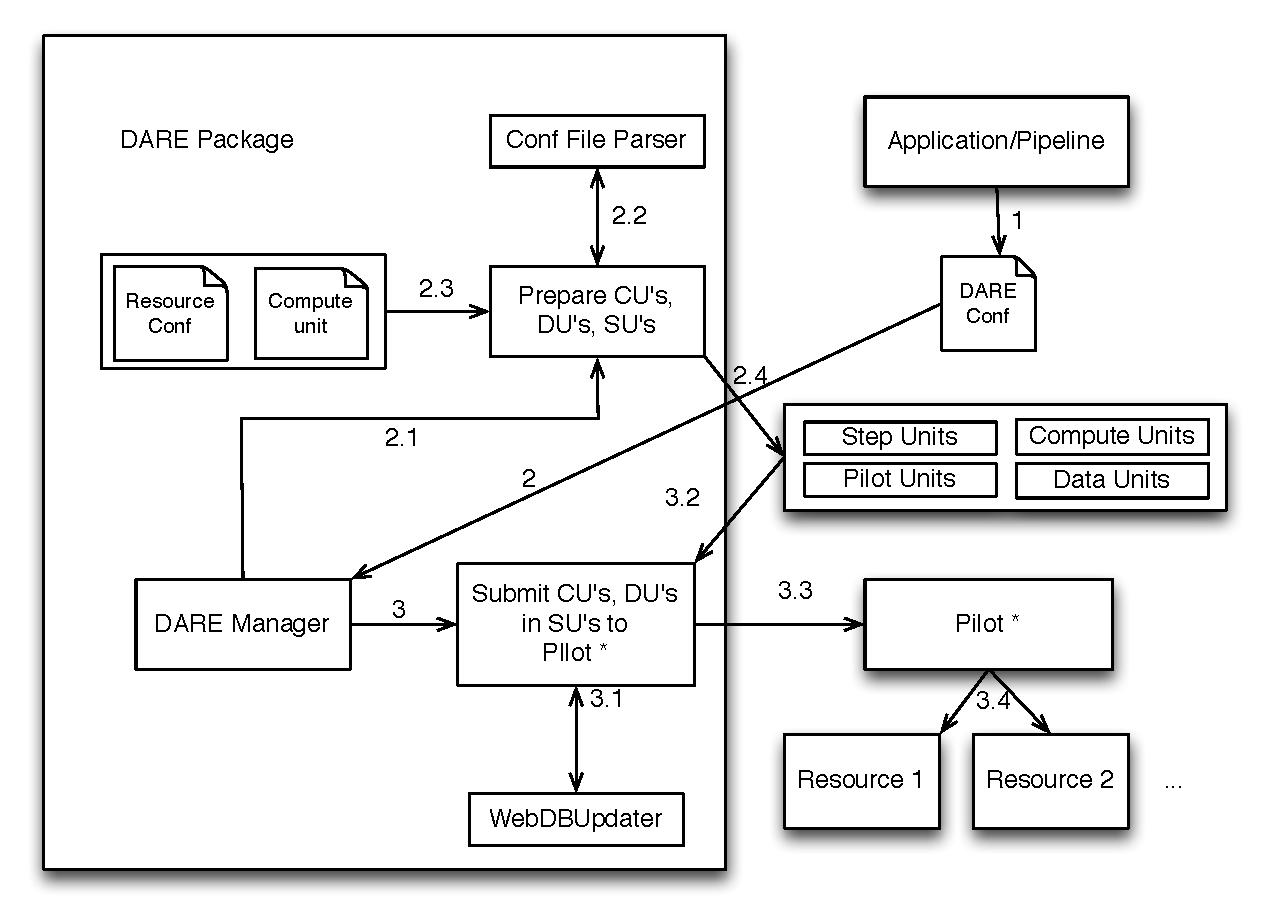
\includegraphics[width=0.66\textwidth]{figures/DARE_Sequence.pdf}
\caption{\textbf{ DARE sequence diagram  }}
 \label{fig:saga-overview}
\end{figure}


\begin{figure}[t]
\centering 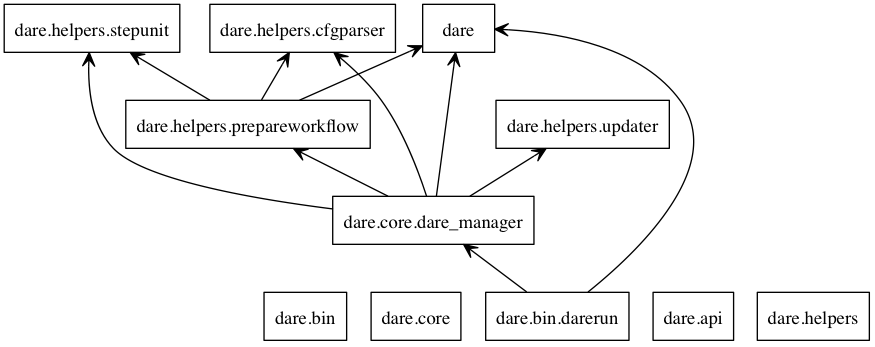
\includegraphics[width=0.66\textwidth]{figures/packages_dare.png}
\caption{\textbf{ DARE Package }}

 \label{fig:saga-overview}
\end{figure}





\begin{figure}[t]
\centering 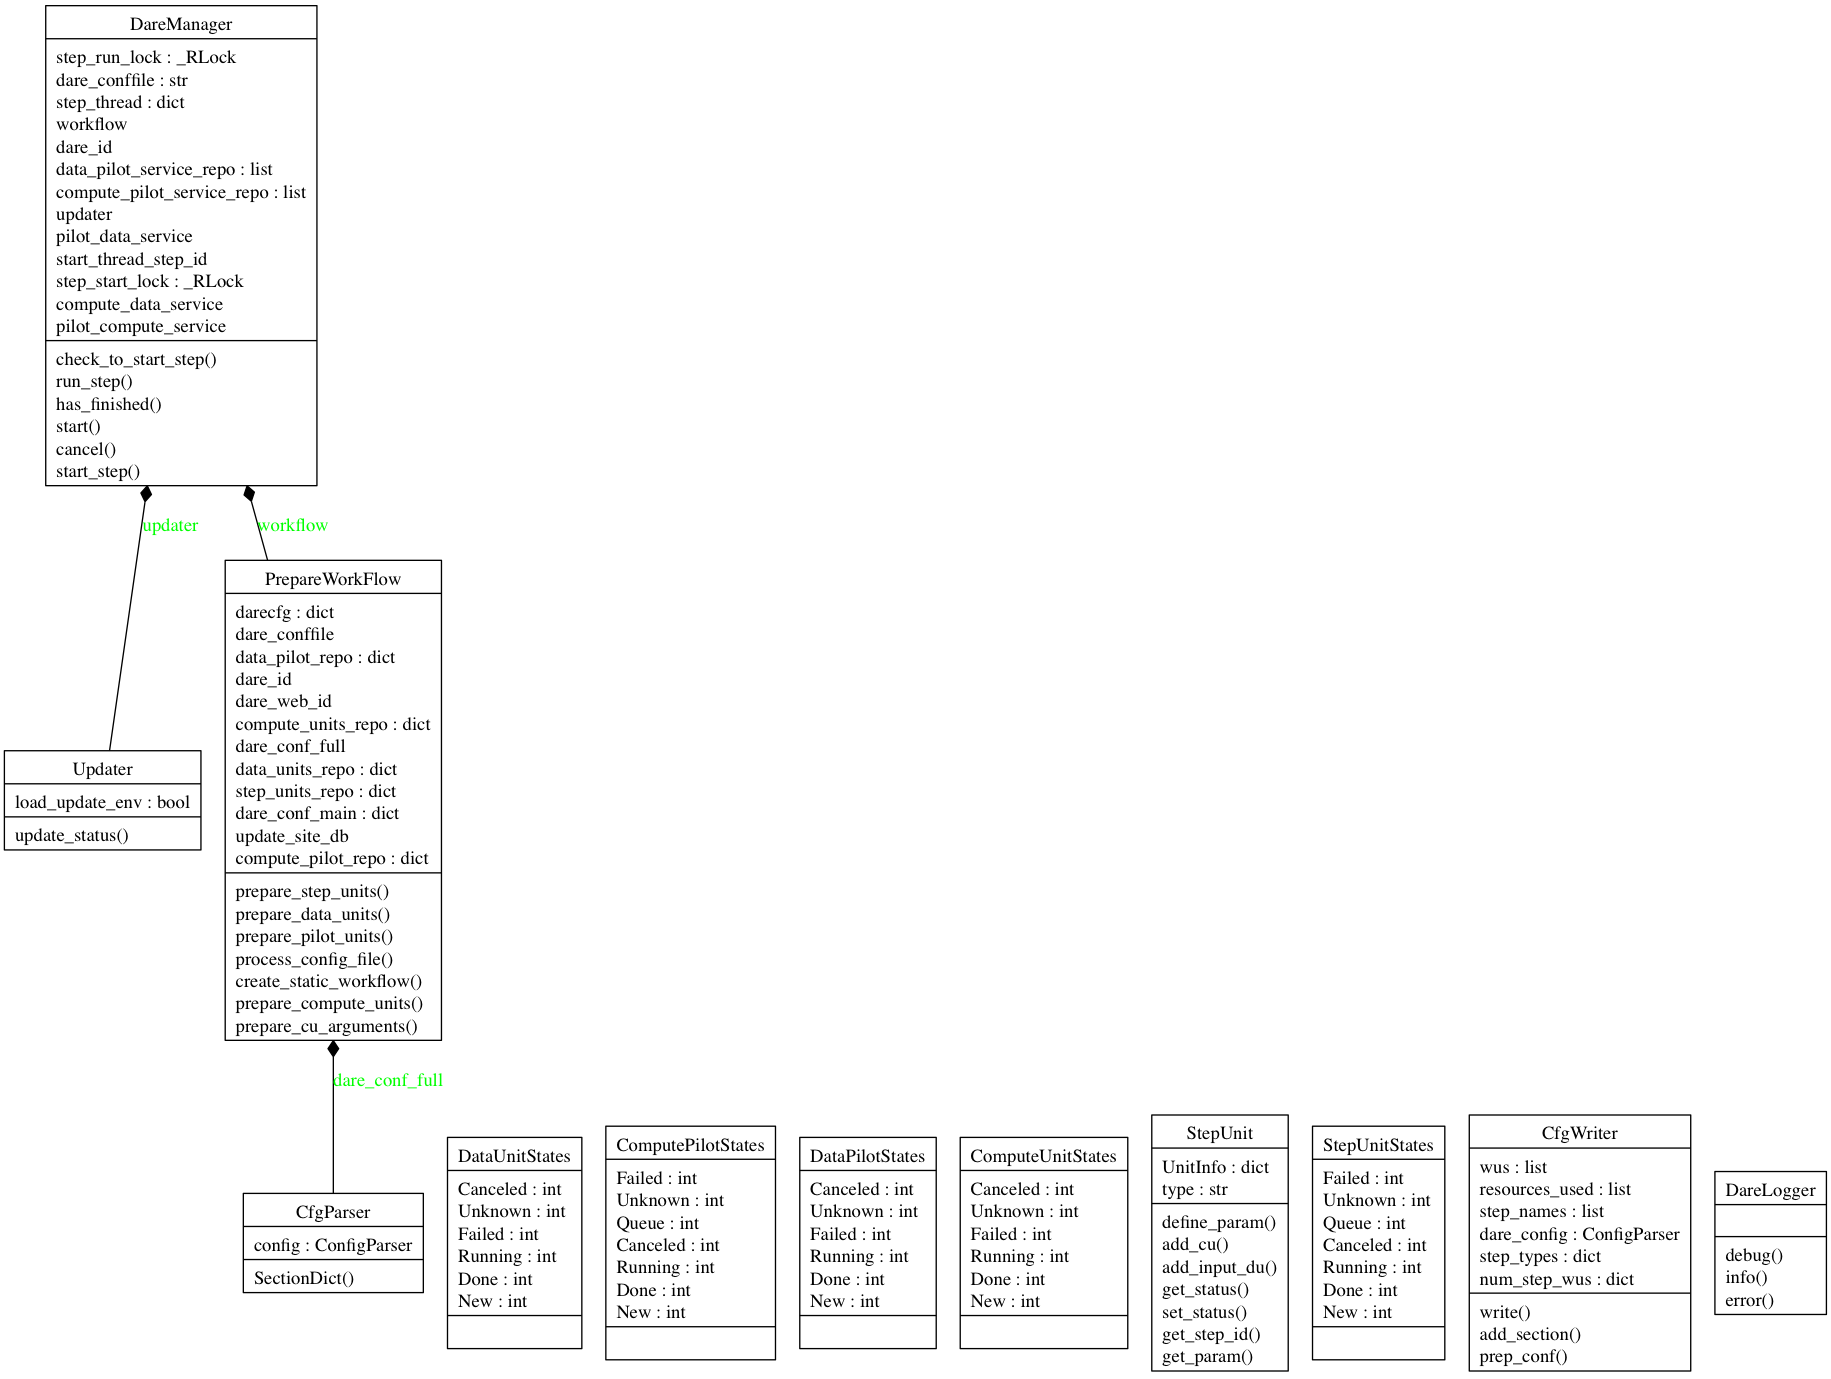
\includegraphics[width=0.66\textwidth]{figures/classes_dare.png}
\caption{\textbf{ DARE classes UML  }}

 \label{fig:saga-overview}
\end{figure}




\subsection{SAGA: Standards-based Access to the Resources Layer}

% SAGA is an API that provides the basic functionality for developing
% distributed applications, tools and frameworks. The key
% advantages of the development using SAGA include, but are not limited
% to: i) to provide a general-purpose, commonly used yet standardized
% functionality, while hiding complexity of heterogeneity of back-end
% resources, ii) to provide building blocks for constructing
% higher-level functionality and abstractions, iii) to provide the means
% for developing broad range of distributed applications such as
% gateways, workflows, application management systems, and runtime
% environments. Interestingly, SAGA provides a simple way to support
% scripting for building distributed applications via python-binding.

\yyenote{The SAGA figure needs to be referenced here somewhere}
\jhanote{please do so! :)} The Simple API for Grid Applications
(SAGA)~\cite{saga_url} is an implementation of an Open Grid Forum
(OGF) Technical Specification that provides a common and consistent
high-level API for the most commonly required functionality to
construct distributed applications. It also provides a high-level API
to construct tools and frameworks to support distributed
applications. The functional areas that are supported by SAGA include
job-submission, file transfer and access, as well as support for data
streaming and distributed coordination. SAGA provides both a syntactic
and semantic unification via a single interface to access multiple,
semantically distinct middleware distributions.

Key advantages to development using SAGA include, but are not limited to:
(i) providing a general-purpose, commonly used yet standardized functionality, while
hiding complexity and heterogeneity of back-end resources, (ii)
providing building blocks for constructing higher-level functionality
and abstractions, and (iii) providing the means for developing a broad
range of distributed applications, and tools to support distributed
execution, such as workflows, application management systems, and runtime environments.

\yyenote{This is sort of backwards: NSF XSEDE operations do NOT
  support SAGA, the SAGA Team supports SAGA, not XSEDE
  consultants.}\jhanote{we're trying to say XSEDE agrees to consider
  SAGA as a software layer becoz of the above mentioned attributes,
  not referencing support} Different aspects of SAGA appeal to
different groups. The standardization of SAGA as an OGF Standard is
important because it makes it more likely that production
infrastructures, like NSF XSEDE and Open Science Grid, will support
SAGA. Having SAGA deployed and tested on these systems makes it
readily available for users and developers of national
Cyberinfrastructure projects. The fact that SAGA is an OGF technical
specification also makes SAGA highly appealing to application
frameworks, services and tool developers, which is quite
understandable, as it not only simplifies their development but also
makes for scalable, extensible and sustainable development. Users find
the simple and extensible interface providing the basic abstractions
required for distributed computing is very appealing to add their own
“functionality” to a core base of functionality. Furthermore, SAGA is
now part of the “official” access layer for the \$121M NSF TG/XSEDE
project~\yyenote{Need to cite XSEDE}, as well as for the world largest
distributed infrastructure EGI~\yyenote{Cite EGI}\jhanote{Yes!}.

The SAGA API provides the base abstractions upon which tools and
frameworks that provide higher-level functionality can be
implemented. Ref.~\cite{saga_url} discusses distributed application
frameworks and run-time systems that SAGA has been used to develop
successfully. 


\begin{figure}[t]
\centering 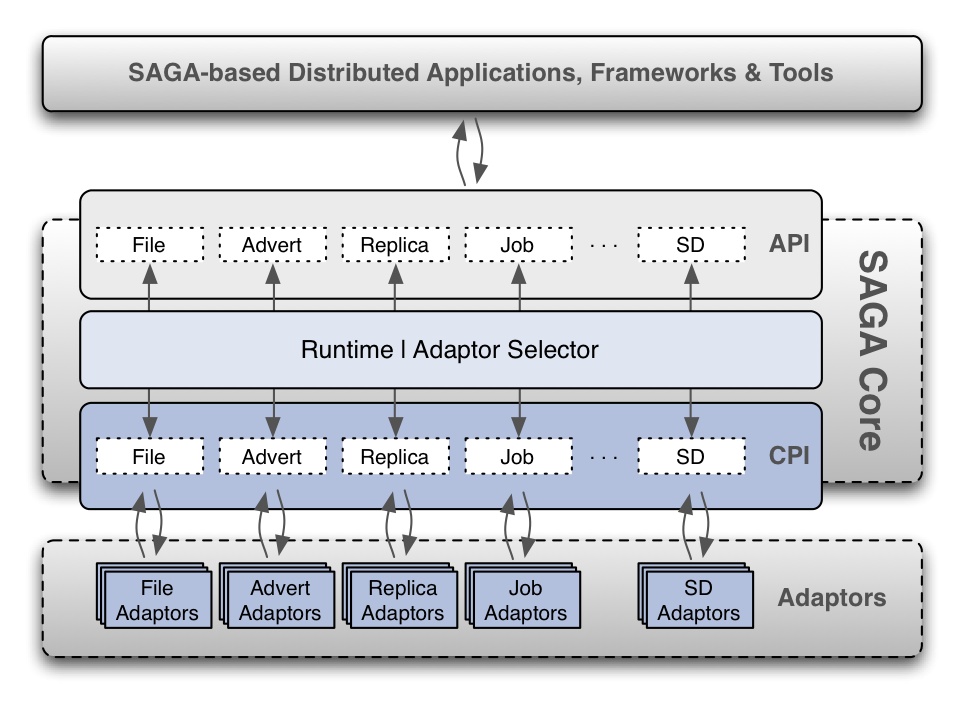
\includegraphics[width=0.66\textwidth]{figures/saga-architecture-1.png}
\caption{\textbf{SAGA Overview: } SAGA is an OGF technical
  specification that provides a common interface to heterogeneous DCI
  -- hitherto typically Grid systems.  The implementation of the
  SAGA\cite{saga_url} specification consists of a high-level {\it
    API}, the SAGA {\it Engine} providing that API, and backend,
  system-specific {\it Adaptors}.  The engine is a lightweight,
  highly-configurable dynamic library that manages call dispatching
  and the dynamic runtime loading of the middleware adaptors.  Each of
  these adaptors implements the functionality of a specific functional
  package (e.g., job adaptors, file adaptors) for a specific
  middleware system. Adaptors are also realized as dynamic libraries.}
 \label{fig:saga-overview}
\end{figure}

A SAGA implementation consists of a high-level API, the SAGA
Engine providing that API, and backend, middleware/systems specific
adaptors. Each of these adaptors implements the functionality of
a functional package (e.g., job adaptors, file adaptors) for a
specific middleware system. The engine is a dynamic library that
manages call dispatching and the runtime loading of the middleware
adaptors. Adaptors are also realized as dynamic libraries. The SAGA
API has been used (in C++, Python and Java versions) to provide almost
complete coverage over nearly all grid and distributed computing
middleware/systems, including but not limited to Condor, Genesis,
Globus, UNICORE, LSF/PBS/Torque and Amazon EC2.

SAGA is currently used on production Cyberinfrastructure in several ways.
Admittedly the number of first-principle distributed applications developed is
low, but SAGA has been used to develop glue-code and tools that are
used to submit and marshal jobs \& data across and between
heterogeneous resources. Specifically, it has been used to support
multiple computational biology applications that use high-performance
and high-throughput molecular dynamics (MD) simulations.

\yyenote{We cannot say saga has been used to develop a science gateway
  in the paper talking about the same science gateway, that is
  circular logic} \jhanote{good point. we need to be careful. this
  paper is about DARE for GW not SAGA. The standards based library
  that we're referring to in the next sentence is actually ARE!} SAGA
has been used to develop a standards-based library for Science
Gateways to easily utilize different distributed resources; some
science domains that are using SAGA-based Science Gateways include
gateways to support next-generation sequencing, docking and
high-throughput of ensembles.

\yyenote{This needs attention. We do not pay attention to pilot-job
  versus Pilot-Job and do not explain the concept clearly}
\jhanote{Someone please look up the macros as defined in the
  pilot-star paper
  \url{https://svn.cct.lsu.edu/repos/saga-projects/papers/troy/pstar/pstar-hpdc2012-acm.tex}
  define here too and then do a global replace/consistency check
  please.}

\yyenote{Need a pilot job definition. No two ways around it. It has to
  be here. Otherwise, the following paragraph needs to be
  removed}\jhanote{provided upstream. ok?}  A prominent example of
such a run-time system is the SAGA-based pilot-job – which provides an
interoperable pilot-job (see next subsection), with consistent
semantics and common usage across different resources. The SAGA-based
pilot-job extends and generalizes the commonly used Pilot-Job concept,
and as a solid validation of the base standards and abstractions that
can be built upon them, has enabled applications to use the same
pilot-job API over hitherto disparate resources for the first time;
advantages include scalability, simplicity and extensibility (of basic
functionality). Similar advantages of scalability, simplicity and
extensibility are now being experienced by Gateway developers as a
consequence of DARE – a SAGA-based library for developing Science
Gateways.


\subsection{DARE: Support for Dynamic Execution and Patterns}
\jhanote{See Fig. 3: DARE is defined as L2 and L3: SAGA + SAGA-based
  Pilot-Job + Patterns (MR) + L2 (Application Capabilities)}

HPDC infrastructure is by definition comprised of a set of resources
that is fluctuating -- growing, shrinking, changing in load and
capability. This is in contrast to a static resource utilization model
traditionally a characteristic of parallel and cluster computing. The
ability to utilize a dynamic resource pool is thus an important
attribute of any application that needs to utilize HPDC infrastructure
efficiently. Applications that support dynamic execution have the
ability to respond to a fluctuating resource pool, i.\,e., the set of
resources utilized at time (T), $T=0$ is not the same as $T>0$.
However, even for traditional high-performance/parallel applications,
the evolution or internal dynamics of an application may vary, thereby
changing the resource requirements. For example, different solvers,
adaptive algorithms and/or implementations, can also require
applications to utilize different set/amounts of resources. Thus, the
need to support dynamic execution is widespread for computational
science applications. In DARE, this is accomplished by building execution
patterns using the SAGA-based Pilot-Job.


\subsubsection{SAGA-based Pilot-Job}

A common approach for decoupling workload management and resource
scheduling, and thereby the dynamic fluctuations inherent in workloads
and resources, is the use of \emph{pilot-jobs (PJ)}. The PJ abstraction is also a
promising route to address additional requirements of distributed scientific
applications~\cite{ko-efficient,bigjob_cloudcom10}, such as application-level scheduling.
 
\begin{figure}[t]
  \centering
%  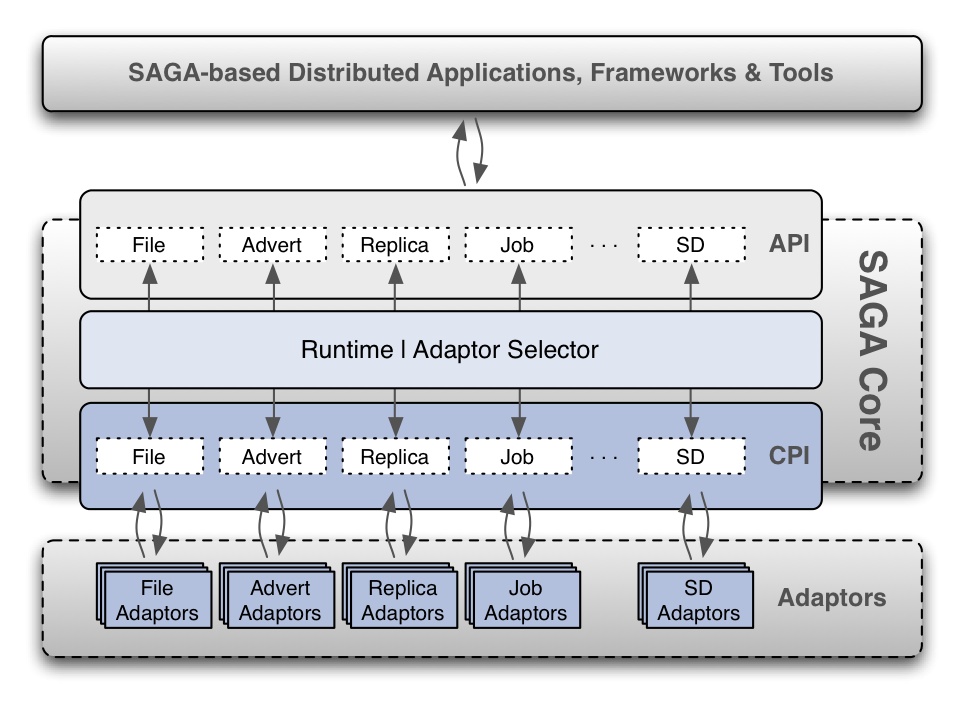
\includegraphics[width=0.48\textwidth]{figures/saga-architecture-1.png}
   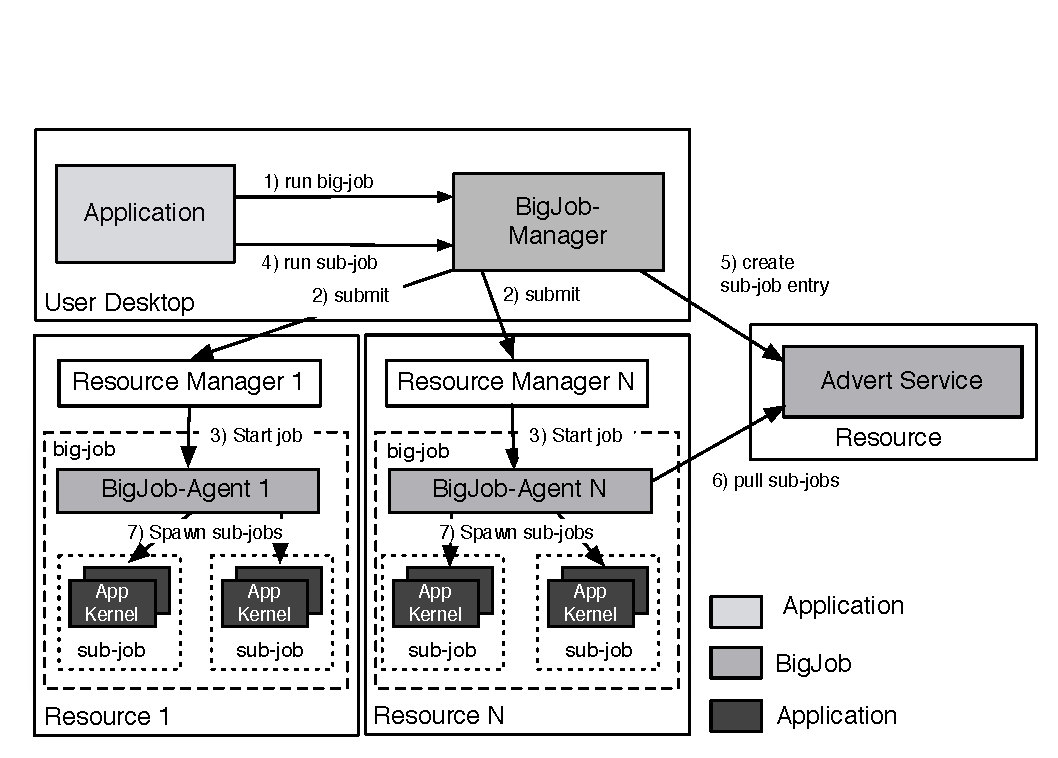
\includegraphics[width=0.48\textwidth]{figures/re_bigjob_interactions.pdf}
  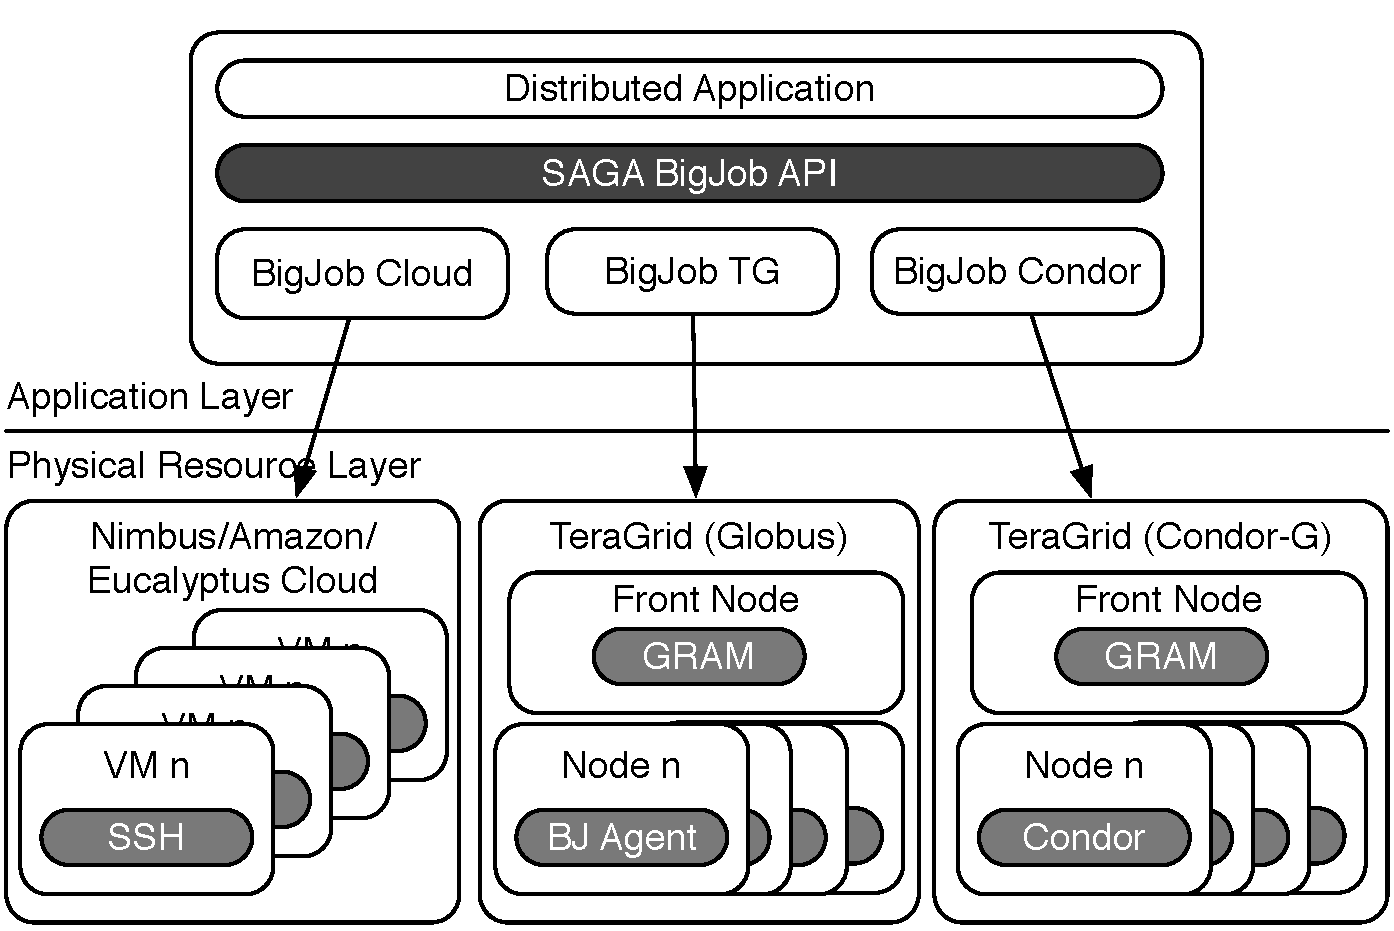
\includegraphics[width=0.48\textwidth]{figures/distributed_pilot_job.pdf}

        \caption{\textbf{BigJob Architecture:} The core of the
          framework, the BigJob-Manager orchestrates a set of
          pilots. Pilots are started using the SAGA Job API. The
          application submits WUs, the so-called sub-jobs via the
          BigJob-Manager. Communication between the BJ-Manager and
          BJ-Agent is done via a shared data space, the Advert
          Service. The BJ-Agent is responsible for managing and
          monitoring sub-jobs. From
          Ref.~\cite{saga_bigjob_condor_cloud}}
        \label{fig:figures_re_bigjob_interactions}
\end{figure}

\yyenote{From Reviewer: This makes it sound as if
BigJob was described in this paper. Maybe reword this a bit to say that it
was described in the referenced papers. Actually, section 2.3.1 reads as if
it describes BJ quite a bit rather than PJ. The last 3 paragraphs of 2.3.1
all talk exclusively about BJ.}\yyenote{Better now}

A SAGA-based PilotJob, BigJob (BJ)~\cite{bigjob_web,saga_bigjob_condor_cloud}, is a
general-purpose pilot-job framework. BigJob has been used to support various
execution patterns and execution workflows~\cite{async_repex11,saga-royalsoc}.
For example, SAGA-BigJob was used to execute scientific
applications categorized as embarassingly parallel applications and
loosely coupled applications on scalable distributed
resources~\cite{ecmls_ccpe10, dare-ecmls11}

Figure~\ref{fig:figures_re_bigjob_interactions} illustrates the
architecture of BJ. BJ utilizes a Master-Worker coordination model. The
BigJob-Manager is responsible for the orchestration of pilots, for the
binding of sub-tasks. For submission of the pilots, SAGA relies on the
SAGA Job API, and thus can be used in conjunction with different SAGA
adaptors, e.\,g.\ the Globus, the PBS, the Condor and the Amazon Web
Service adaptor. Each pilot initializes a so called BJ-agent. The
agent is responsible for gathering local information and for executing
tasks on its local resource. The SAGA Advert Service API is used for
communication between manager and agent. The Advert Service (AS)
exposes a shared data space that can be accessed by manager and agent,
which use the AS to realize a push/pull communication pattern.
The manager pushes a sub-job to the AS while the agents periodically pull
for new sub-jobs. Results and state updates are similarly pushed back from
the agent to the manager. Furthermore, BJ provides a pluggable
communication \& coordination layer and also supports alternative c\&c
systems, e.\,g.\ Redis~\cite{redis} and ZeroMQ~\cite{zmq}.

In many scenarios it is beneficial to utilize multiple resources,
e.\,g.\ to accelerate the time-to-completion or to provide resilience
to resource failures and/or unexpected delays. 
BJ supports a wide range of application types, and is usable over a
broad range of infrastructures, i.\,e.\ it is general-purpose and
extensible (Figure~\ref{fig:figures_re_bigjob_interactions}). In
addition there are specific BJ flavors for cloud resources such as
Amazon EC2 and Microsoft Azure that are capable of managing set of
VMs, as well as a BJ with a Condor-G based backend.

BJ supports dynamic resource additions/removals as well as late
binding. The support of this feature depends on the backend used. To
support this feature on top of various BigJob implementations that are
by default restricted to single resource use (e.\,g.\ BJ), the concept
of a BigJob pool is introduced. A BigJob pool consists of multiple BJs
(each BigJob managing one particular resource). An extensible
scheduler is used for dispatching WUs to one of the BJs of the pool
(late binding). By default a FIFO scheduler is provided.

\yyenote{SJ check the following} \jhanote{yes, this is weak and needs
  attention} All user side aspects of BJ can be provided to end-users
in a science gateway through DARE. Science gateway developers can
expose as little or as much of BigJob as needed to the end-user as
well as expose functionality for users to create workflows. Some
commonly used workflows have already been built into DARE. These are
referred to as pattern-based execution models.

\subsubsection{Support for Patterns-based Execution}

There are several common workflows required for multiple life-sciences
applications. These workflows include launching ensembles of simulations
or pipelines consisting of application execution followed by analysis.
These workflows can repeat any number of times and can include
data-management or analysis stages. We refer to these common workflows
as workflow patterns: general templates frequently used in life sciences
applications. DARE supports some of the well known patterns such as MapReduce
and Scatter-Gather. DARE also supports launching of large ensembles
of loosely-coupled or uncoupled tasks. \yyenote{Check the previous statements}


DARE's support for these common patterns is generic, and thus easily
adaptable to many different applications (not necessarily life sciences).
In section \S3 we will discuss some of the common patterns available
in DARE. The support for a patterns-based execution is a useful and novel
feature of DARE. Although not all of these are fully developed,
a large number of execution patterns are already supported, e.g,
uncoupled and loosely-coupled ensembles, Master-Worker, MapReduce etc.

% A recent and novel feature is that support for execution patterns are
% not limited to computational tasks alone, but also to data-access
% patterns.  Full details are beyond the scope of this paper, but
% support for data-access patterns and compute execution patterns are
% implemented in an integrated fashion thanks to the common treatment
% via the pilot-job and pilot-store capabilities provided by SAGA-based
% P* model~\cite{pstar11}.  For example, the Pilot-Job/Data provides a
% natural abstraction to support MapReduce based
% applications~
% \cite{saga_data_intensive_abstractions,Sehgal2011590,fgcs-interop11}. The middle
% layer of L3 (Runtime
% System) in Figure 5 illustrates the combined and integrated
% computational tasks and data capabilities.


% Multiple approaches exist to support dynamic resource utilization, for
% example, advanced scheduling (without pre-emption) provides
% essentially a guarantee of resources at a sufficiently far out time
% window.  However, distributed applications that are able to break the
% coupling between workload management and resource
% assignment/scheduling have been successful at efficiently utilizing
% distributed resources, without the policy-level complexity of
% implementing advanced reservations. 


% In Fig.~\ref{fig:dare-arch}, we present the architecture of a
% gateway based on the DARE-framework; it is comprised of the four
% layers : (i) User Interface, (ii) Applications, Capabilities and
% Services, (iii) Runtime Environment, and (iv) Resources. Note that
% this schematic emphasizes primarily our own integration strategy
% around the layer L3, that is built with the DARE framework, to
% bridge resource utilization and user interactions. Other aspects
% that are required in a typical Science Gateway are not explicitly
% shown or simply ignored.  Also, it is noted that the schematic shows
% clearly that underlying development mechanisms are independent and
% modular, but effectively connected to each other under the
% framework. More details will be discussed later in conjunction with
% Science Gateway development.


% \subsection{Putting it together: 


%\subsection{DARE: A Framework for Science Gateway Development}


\section{DARE-based Science Gateways: A Four-layer Architecture}

%\subsection{Four Layers Architecture of DARE-based Science
%  Gateways}

\begin{figure}
  \centering
  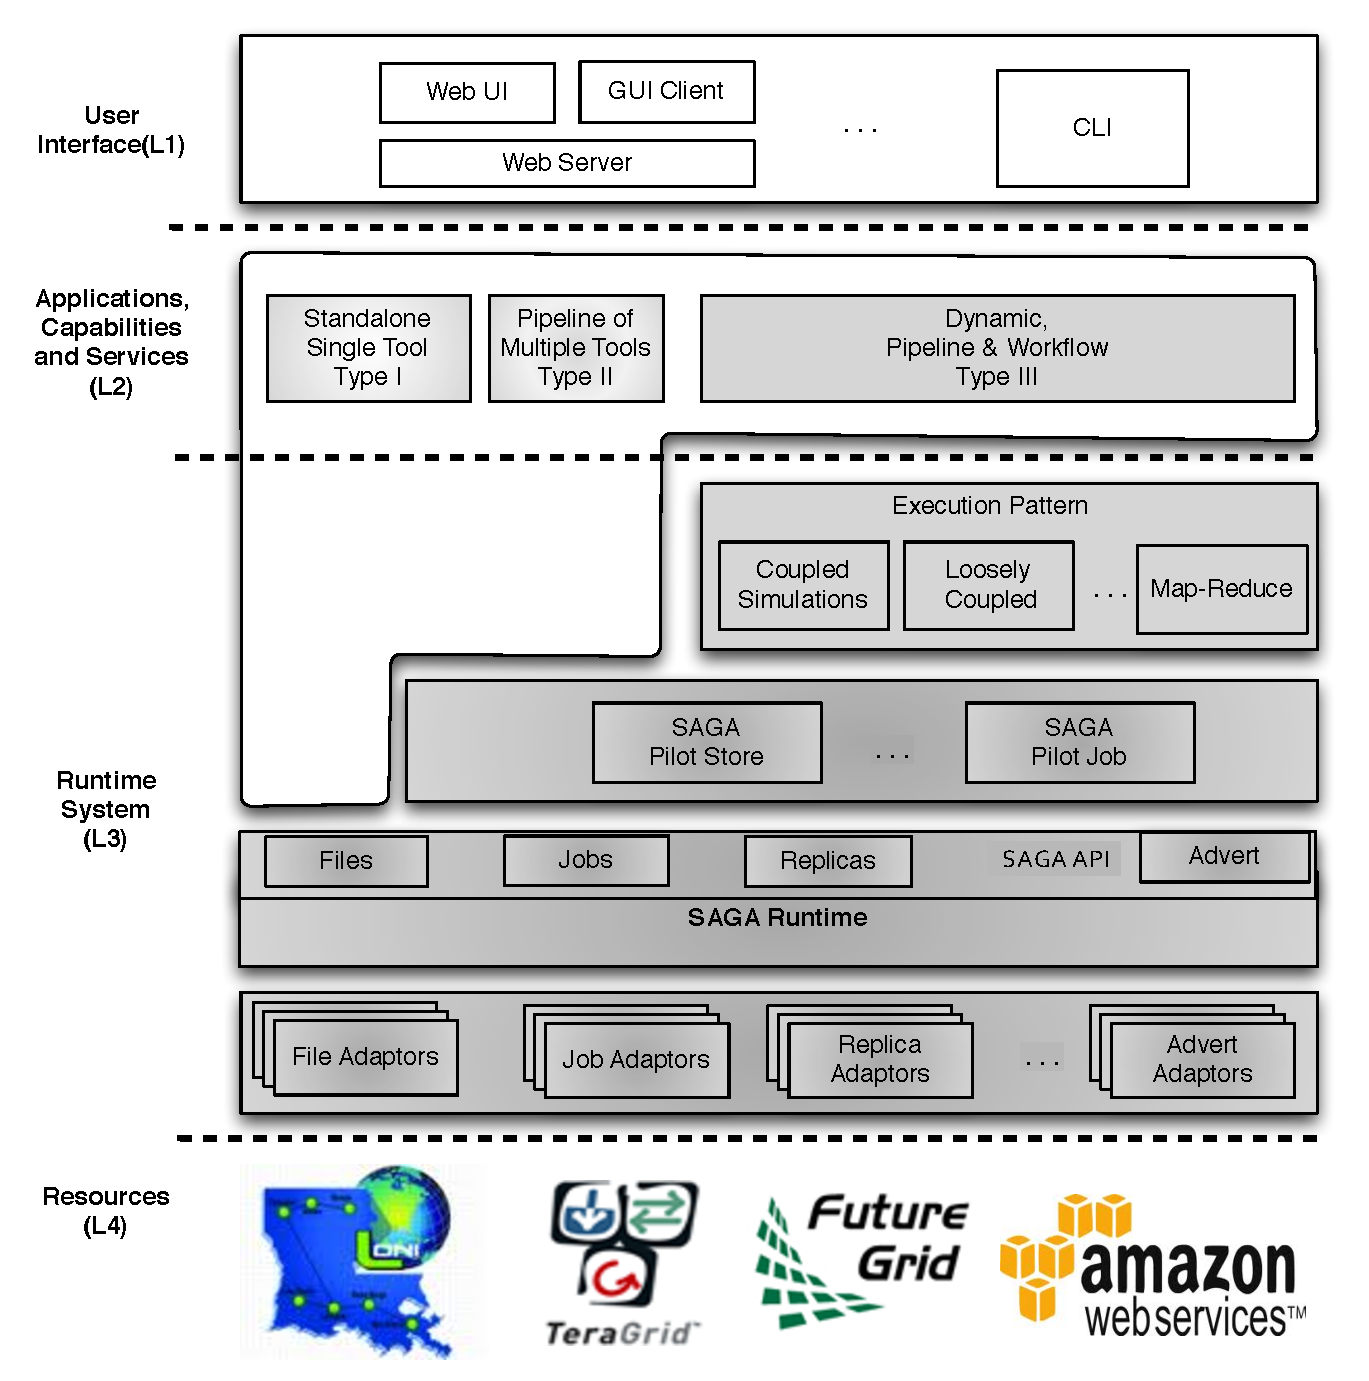
\includegraphics[scale=0.55]{figures/DARE-gateway-arch.pdf}
%  \includegraphics[scale=0.30]{figures/DARE-gateway-alt.png}
  \caption{\small \jhanote{Use updated figure} Overall architecture of a DARE-based gateway comprising four levels. % (right) An illustration of a different view of a DARE-based gateway architecture
  }
  \label{fig:dare-arch} 
\end{figure}


%{\it DARE-based Science Gateways: Four-layered Architecture: }

As illustrated in Fig.~\ref{fig:dare-arch}, a typical gateway needs a
user interface for everything from authentication and authorization
to the ability to submit user requests, jobs, and data management. 
Ideally these capabilities are implemented as integrated middleware on
a range of hetrogenuous compute resources. The user interface simply
interfaces the middleware, glossing over details of function calls,
language syntax and so on.

% \yyenote{The following sentence needs improvement: what do we mean by
%   maximizing the capacity of DARE?}\jkimnote{i made a change} 

% A design strategies of the gateway development suggested in
% Fig.~\ref{fig:dare-arch} is to maximize the strength of DARE for
% gateway applications.

Thus DARE based science gateways are typically organized in levels.
Levels L2 and L3, are common to all gateways, and are decoupled from
access level (L1) and resource layer (L4). Development is therefore
modular and layered. Adding support for a new resource, for example
OpenStack based clouds in L4, is as simple as adding the required SAGA
adaptors in L3. No changes need to be made at L1 or L2. Similarly,
adding more execution patterns and workflows in L2 is decoupled
from the runtime system in L3 and the resources involved in L4.

% Additionally, the development and
% implementation of a broad range of execution patterns that are
% facilitated by pilot abstractions for distributed tasks and data are
% effectively achieved (which are the core features from DARE levels,
% L3) without knowing the details of high- level characteristics of
% services that is solely defined in L2.

\subsection{User Interface Level ($L1$)}
% \yyenote{The paper is about web based science gateways. We should not be talking about the command line}
% \jhanote{I think this entire paragraph can go?} Depending upon the
% type of UI, i.e. Web-based or vanilla command line UI, three-tier or
% two-tier gateways are possible. For example, if access mechanism is
% through a web browser or a remote client, the overall architecture
% could be built as a three-tier architecture in which a user desktop, a
% server that contains middleware comprising L2 and L3, and back-end
% resources are independent to each other. Currently, the use of web UI
% is a default for a user access. On the other hand, if Command Line
% Interface (CLI) is preferred, the overall architecture would be
% two-tier, since there exists no need of a system for a remote user.
The current prototype web user interface is built on top of
Pylons~\cite{pylons_website}. The Pylons project is a collection of
Python based web frameworks that are lightweight and easy to use. Pylons
uses the common Model-Viewer-Controller design pattern and is written
in Python and thus easily interfaces with DARE. Pylons handles everything
from user authentication, database creation/management,
and data storage/retrieval. Creating a user interface is straightforward
and ``connecting'' the user interface to the server-side services in DARE
was surprisingly simple.


% Using pylons benefits primarily with its
% full-fledged web application framework capabilities allowing
% lightweight, extensible, and efficient web technologies, which is
% hardly achievable with other various Java-based approaches and other
% web application frameworks that might be more powerful but unnecessarily
% heavyweight for tasks required for Science Gateways. 
% Compared to them,
% pylons is widely proven with its efficacy for building a web
% application and high-quality features for a web application~\yyenote{Any citation to this? it is a bold claim and needs some support}.

% The
% Model-View-Controller (MVC) architecture model that underlies the
% pylons web application framework \cite{bigjob_cloudcom10} is very effective
% and advantageous in many ways. For example, database creation,
% management, and transaction are extremely simple and robust to
% facilitate authentication steps and job/data creation and management
% by storing or retrieving related data. Additionally, UI
% creation/development and the connection between server-side services
% (provided by the Services Layer) and UI-based user interactions are
% also surprisingly simpler compared to other existing approaches,
% requiring less programming efforts. For example, it is well
% appreciated that for a science gateway development, the utilization of
% databases and server-side programming are non-trivial tasks~\yyenote{previous sentence is awkward. Did this appear somewhere else and was lifted for this section}. Finally,
% its python root is a plus factor that is easily integrated into the
% middleware including DARE core that are also written as python
% scripts.


\subsection{Applications, Capabilities and Services Level ($L2$)}

% \yyenote{what does the following even mean}
% It is a developer's responsibility to find the optimal logic,
% usage-mode for the target scientific application.

The application layer implements the logic necessary for pattern
execution. In other words it implements the logic necessary to
create jobs of single standalone applications, piplelines and
dyanmic workflows. It does not run scripts on resources but is
a necessary abstraction over the actual runtime systems. 

The application layer is where execution patterns are prepared for the
runtime system to execute. Three categories of patterns are available
to users, Types I, II and III. Type I is the simple, standalone tool. 
Type II is a linear pipeline of tools and type III is a dynamic workflow.
A combination of early life sciences focus and gradual development
led to this categorization. It is also a natural and convenient
breakdown of available services.

% The Application Layer's role is to support this responsibility, i.e., implementing the
% logic and usage-mode. Thus it is an important component of the
% development and uptake of the gateway. As we will discuss, the
% middleware Levels (i.e. L2 and L3) also mitigates developmental
% hassles due to reliance on DARE, i.e. the SAGA/SAGA-based runtime
% environment framework.

% The services provided by the gateway and their implementation of
% execution patterns and distributed modes for tasks and data are
% decided with L2. Note that the development of this level varies with
% target services, but could be efficient by abstracting various
% execution patterns and task/data management that constitute
% collectively the execution of dynamic applications. Such abstractions
% are implemented in L3 and facilitate the development of
% L2. Furthermore, we categorized into three kinds of services (Types,
% I, II and III), based upon level of complexity, scientists' usage
% mode, and required software tools associated with the services
% provided via the DARE-based gateway, which provides the starting point
% of a target service with its general characteristics. In other words,
% this categorization also reflects characteristic features of such
% services with respect to execution patterns of tasks supported by
% DARE.

\begin{table}[!h]
\centering
\begin{tabular}{| l | l | l | l |} \hline \rowcolor[rgb]{0.8,0.8,0.8} &
Type I & Type II & Type III \\ Description & Standalone  & Pipeline & Workflow-based \\ 
& Single Tool  & or Multiple Tools &  \\\hline 
% Target Tool Modification & Not Needed &
% Not Needed & Minimally Needed \\ \hline Scientific Workflow & Not Needed & Useful but Not Necessarily &
% Needed \\ \hline 
NGS Example & BFast, BWA,  & MACS, TopHat-Fusion,  &   Novel Service for 
 \\
 &  Bowtie, ABySS  & TRANS-ABySS, Hydra & RNA-Seq \\
\hline
\end{tabular}
\caption{Comparison of three kinds of services provided by the
  DARE-based gateways. The lower row provides specific examples of
  services  implemented for NGS analytics as part of DARE-NGS.}
\label{table:three-type-service}
\end{table}

% In brief, Type I \& II represent services that enable a user to run
% either: a standalone application, an independent execution of
% multiple tools, or a pipelined execution of multiple tools.

% \jhanote{Most of Tools in tables~\ref{table:four-applications} and
%   ~\ref{table:three-type-service} irrespective of their provisioning
%   as Type II/III are provided as a minimum as a Type I service}.

Table~\ref{table:three-type-service} shows some of the common life sciences
applications currently being used and their respective pattern types. All
of these applications can be used independently as standalone Type I services.

In general, a program developed as a single standalone application needs
less effort and is in many cases straightforward to integrate with
DARE. These are typically provided as Type I service. In contrast,
Type II services are built by incorporating different individual
tools/applications, and linked so that the output of one is
pre-determined as the input of another, i.e., provided as pipelines.
Making a pipeline available as Type II services provides
two major advantages: availability of multiple tools that are used in
conjunction with each other in one location, and the enhanced
capability to utilize scalable resources such as TG/XSEDE and other
HPC and Cloud resources.

On the other hand, Type III services aim to support more complex
service, both in the type of workflows supported as well as more
sophisticated execution. In contrast Type I and Type II
services aim to serve stand-alone and pipelined tools with
advanced cyberinfrastructure capabilities, scalable production infrastructure and
integrative efficient pipelines. They are however limited to static execution:
once the job submission scripts are in, nothing can be changed.

Additionally, pipelines offered as Type II may often require greater
runtime flexibility, i.e., different stages may run on different
resources which may not be determined until execution time; these
``dynamic'' Type II pipelines will be thus offered as Type III
services. The specific resources that are utilized in the
execution phase are determined dynamically -- either through delayed
binding or are refined/optimized after the initial resource
assignment.

Type III Scientific workflows with dynamic execution are possible with
these DARE features. Type III workflows are fully customizable and
extensible, whereas Type II workflows are predefined and used as is.
Type III services obviously can run Type II workflows.

% To support these additional features, a Type III  scientific
% workflow with which a rapid development of dynamic execution
% patterns is possible. Workflows of Type III are customizable and
% extensible, whereas a workflow of Type II is predefined; Type III
% services can also invoke the ever-increasing concrete Type II
% services.

\subsection{Runtime System Level ($L3$)}

L3 represents the core of the DARE framework. In a nutshell, it
integrates the application-level capabilities (L2, support for Type
I/II/III services) with the HPDC infrastructure (resources/L4) layer. The DARE
runtime level in turn achieves this via a critical dependence on
SAGA. The challenges in building a scalable distributed gateway are
greatly mitigated by SAGA and/or SAGA-based frameworks. The
SAGA-runtime system has the responsibility to make middleware specific
dispatches.

% DARE exposes support for a range of execution patterns, which in turn
% can use the pilot-job/data abstractions. Application-level
% capabilities can be provided via these execution patterns, or use the
% pilot abstractions directly; or possibly use the SAGA
% job/file/replica/advert functionality directly.

% and we describe here some backgrounds for its development and the
% relation with SAGA and SAGA-based pilot job abstraction, SAGA-BigJob.
%For example, by varying SAGA-BigJob configuration, 

The SAGA-BigJob supports dynamic configuration changes, thus it is
relatively easy to optimize the usage of target resources for a given
computational workload and their execution characteristics. Examples include
embarassingly parallel, loosely-coupled, or even multiple instances of
tightly-coupled applications. Thus once the desired configuration has
been determined, a gateway developer can easily construct an optimized
runtime environment for a given target application capable of
utilizing distributed resources without any application or
infrastructure refactoring.

Furthermore, it is important to consider data movement requirements,
since the movement of large data sets (input, output, and temporary
files) is a major challenge. We have recently analyzed the
date-volumes that need to be moved around, and demonstrated some of
the challenges and solutions for BFAST~\cite{dare-ecmls11}, an NGS
application prototype~\yyenote{What was the conclusion of the analysis
  of the challenges and solutions from BFAST. Can somebody add a
  sentence here saying what we concluded please}.\jhanote{Joohyun,
  please comment/add from the TG'11/ECMLS paper please} At the moment,
GridFTP and scp are used as the primary protocols for data
transfer. Support for Globus-Online is imminent. As we will discuss in
\S4, typical data-volumes for NGS applications can easily exceed
100GB; data-movement services need to and can managed these
volumes.~\yyenote{I am keeping the previous sentence but do we
  actually make good on this promise. Where do we disucss this in the
  paper. Please confirm}\jhanote{Good point. We do have support for
  Globus Online now in Pilot-Data. BTW need reference to Globus
  Online. Also, we should generalize to advanced data-transfer
  protocols in addition to GO}

It is worth noting that SAGA supports different transfer protocols
along with data-intensive programming models such as MapReduce.
Thanks to the dynamic adaptor loading mechanism, SAGA can provide
these execution patterns for emerging data intensive computing
infrastructure such as clouds~\cite{bigjob_cloudcom10,saga_bigjob_condor_cloud}.

%  Traditionally, frameworks are limited to specific patterns or to
%  specific platform implementations. In short, they lack generality, as
%  shown by a team working with HiMach~\cite{deshaw_sc09}, a
%  MapReduce-based solution for analyzing molecular dynamics trajectory
%  for petascale distributed data.  They found that minor extensions to
%  and a different usage model of MapReduce rendered existing MapReduce
%  implementations unusable on their platforms (not Hadoop)
%  and required the creation of new runtime frameworks and application
%  support.

% In Figure~\ref{datefig}, we present a layered framework approach for
% achieving the... 




% This work presents four different gateways for different life-science
% applications, once 

% One figuring out preferable application usage modes as
% well as parallelization strategies, 

% The web interface will be connected to remote job submission via a
% job scheduling and monitoring thread. This thread starts with pylons
% application and continuously communicates with local database server
% to find new jobs and it also acts as a scheduler for new jobs. Once
% this thread finds a new jobs it will start preparing the
% configuration files for that particular job from the user and
% afterwords it will start the remote job submission via application
% specific SAGA-Bigjob.
%should be carefully considered when a gateway is developed,


% All the above components are well connected but loosely coupled from
% each others as well so this provides the development of different
% kinds applications very simple and fast.

\subsection{Resources Level ($L4$)} 

While the utilization of distributed heterogeneous resources should be
one of the important motivations for a science gateway
development~\yyenote{No. Why should it be?  The important movitation
  in science gateway development is to simply the interface to compute
  resources. The fact that dare supports distributed runs is a bonus,
  not a primary motivation.}, \jhanote{The two objectives are not
  mutually exclusive, i.e., the simple interface versus the back-end
  access to infrastructure} most gateways currently rely on the
approaches in which multiple resource utilization is limited,
presumably, only for supporting embarassingly-parallel multiple
tasks.~\yyenote{I say delete all the previous paragraph} \jhanote{I
  think it actually can stay given that this is L4}

SAGA and SAGA-based frameworks enable distributed scale-out across
multiple production grade resources.  These production grade resources
include grids of large systems such as Ranger, Kraken and Lonestar as
well as HPC clouds on FutureGrid and vendor solutions such as Amazon's
EC2. A basic design principle that the runtime system adheres to is
future-proofing through extensibility and abstraction. When adding a
new computing platform, only a small amount of code has to be written
as a SAGA adaptor to enable access to that platform.

To cement support for different resources in L4, SAGA was deployed
publicly on XSEDE. The installations are available for anyone and everyone
to use: no private or shared accounts, no special permissions. Ranger,
Lonestar, Kraken, Trestles, Steele as well as most FutureGrid machines
have SAGA installations that are maintained and kept up to date by
the SAGA team and supporting XSEDE personnel. Furthermore, several virtual machine images with
SAGA installations are available publicly on EC2. Any science
gateway developer can in principle and practice use these installations
for their DARE based science gateway.


% Various SAGA adaptors contribute to achieve interoperability for
% inter-HPC-grids, HPC-cloud, and other hybrid resources. There is also
% the capacity to develop new developers complete with full
% documentation~\cite{saga_url}.  In addition, SAGA-BigJob adds the
% capability to support various adaptive executions as already shown
% with scientific applications such as Replica Exchange Molecular
% Dynamics, hybrid CFD-MD, and NGS data
% analytics~\cite{saga-royalsoc,ko-efficient,dare-ecmls11}.


% \jkimnote{the following paragraph needs to be shorten or moved into
%   the Services Layer?}  The access layer is connected to service layer
% with the help of configuration files. The job-scheduling/monitoring
% thread which starts along with the web server is responsible for
% writing the job configuration file which changes for every single
% job. Apart from this job configuration file there are two other
% configuration files, first one has the resource list which is common
% for any application (DARE-NGS, DARE-HTHP etc. ) and the other one is
% application specific configuration on each resource containing the
% paths for executables, input, output directories. once the
% job-scheduling/monitoring thread creates the job specific
% configuration file, it invokes another thread which starts reading the
% configuration files assigned to it and acts as a manager for this
% particular job. And this thread is responsible for transferring the
% appropriate input files to different resources, submitting and running
% the required jobs requested by user and getting back the output files
% which are in turn zipped and provided to user for download via
% web. But , we have keep in mind the uploading input files and
% downloading output file via web browser has not been implemented since
% the files sizes are too big to handle via browser and we are working
% on finding ways to handle this kind of situation. SAGA plays an
% important role with this job manager thread which makes the remote job
% submission and files/folders movement across different machines very
% simple and easily usable.

 \section{EXAMPLES OF DARE-BASED GATEWAYS FOR LIFE SCIENCES}

\jhanote{Some text here..}

\subsection{DARE-NGS}


\begin{table}
\centering
\scriptsize
 \begin{tabular}{|c|c|c|c|c|c|c|} 
 \hline 
Genome & Index         & Resource    & \# of & \# of &   \# of         &	TTC  \\
  Type               & File (GB)        & &Cores &   nodes &  VMs&  (sec)\\  
  \hline
 BG &0.435& R&	64 &4&-	&1067 \\
\hline                  
BG &0.435& QB	&	64& 8&-	&719 \\
\hline
 BG &0.435&R/QB	&	32/32 &2/4& -&919 \\
\hline
 BG &0.435& FG &	64 &-&8	&712 \\
\hline
 BG &0.435 &  R/QB/ &	24/24/& 2/3 & 3 &1022\\
 & & FG& 24 &&&\\
\hline
\hline
Chr &1.9& R	&	64& 4 &-&1145 \\
\hline
Chr &1.9& QB	&	64&8&-	&924 \\
\hline
Chr &1.9& R/QB	&	32/32& 4/2&	-&1170 \\
%\hline
%HG18-Chr21 &1.9& FG	&	64	& \\
%\hline
%HG18-Chr21 &1.9& R/QB/FG	&	24(2),24(3),	& \\
%&& 	 &24(3)&\\
\hline
\hline
HG &127& R	&	256 & 16 &-	&9586\\
%\hline
%HG &127& QB	&	256 &32 &-	& \\
\hline
HG &127& R/QB	&	128/128&8/16 & -&7582 \\
\hline
\end{tabular}
\caption{
  Comparison of Time to Completion (TTC) required for the NGS data
  mapping calculations using BFAST (match step) using DARE-NGS. 
  Three genome types,
  HG18 (HG), HG18-Chr21(Chr), B. Glumae(BG) represent a human genome,
  chromosome 21 of HG18, and the genome of a microbe Burkerholderia
  Glumae. Three compute resources are Ranger (R), QueenBee (QB), and
  FutureGrid  Eucalyptus Cloud on Sierra (FG), respectively. The
  number of tasks for carrying out the required mapping calculation is
  30(135MB) for B. Glumae and 32(169MB)for HG18 and HG18-Chr21.
}

  \label{table:NGS-Distributed} 
\end{table}

The DARE-NGS gateway % (\url{http://dare.cct.lsu.edu/gateways/ngs})
is a prototype gateway built upon the DARE framework and focusing on
Next-Generation Sequencing data analytics and downstream analysis; it
currently supports the mapping process using BFAST, BWA, and Bowtie
and other pipelines for RNA-Seq and
ChIP-Seq\cite{mardis2008-arghg,ecmls_ccpe10}. Mapping (alignment) is
the first step in scientific discovery utilizing NGS sequencing-based
protocols including the whole genome resequencing, RNA-Seq, and
ChIP-Seq.

Recently, we investigated the mapping step using BFAST, one of a new
generation alignment software tools. BFAST aims to provide higher
sensitivity, rather than be optimized for computational efficiency
(which is the design objective of most other popular aligners).
% a software tool
% to aim high sensitivity rather than compute efficacy that is
% previously favored by popular aligners. 
It is worth mentioning that the computational complexity of the
analysis (e.g. mapping) depends, upon other things, on the size and
complexity of the reference genome and the data-size of short reads,
but mostly algorithms\cite{dare-ecmls11}.  Our investigation of the
computational requirements and efficient concurrency supports for
data-intensive BFAST mapping led us to conclude that, given that these
can vary significantly, the computational requirements of
NGS-analytics also varies (even between data-sets of similar
size). Thus an efficient, scalable and extensible analytical approach
must be supported by any framework supporting NGS-analytics.

%\begin{figure}
% \centering
% \includegraphics[scale=0.40]{figures/dae-rfold-result.pdf}
%\caption{\small Massive concurrent calculation capability is presented with the results obtained with DARE-RFOLD. The total 2910 SAM-I riboswitch sequences are injected into the DARE-RFOLD for sampling of Boltzman-weighted secondary structures. SAGA-BigJob handles these many tasks by decoupling the resource assignment and execution of each task, collectively allowing an efficient management of many tasks. In (a) and (b), time-to-solutions with different configurations of BigJob are compared in terms of the number of BigJobs (a) and the size of a BigJob (b). In (c), the distribution of sizes of 2910 input sequences is illustrated. This distribution is directly associated with the distribution of time-to-solutions of all 2910 tasks. The data are taken from the recent work\cite{ccpe11}.}
%  \label{fig:dare-rfold-result} 
%\end{figure}

As an example of L2 for DARE-NGS, Table~\ref{table:three-type-service}
provides simple overview of the three types of services.
NGS analytics using DARE-NGS on HPC grids such as TG/XSEDE and Cloud
environment of FutureGrid were conducted\cite{dare-ecmls11}. Using the
results obtained from such an effort, we present the comparison of
various execution scenarios with multiple resources including a cloud
system in Table~\ref{table:NGS-Distributed}. 

While this demonstrates the capability of DARE-NGS for utilizing HPC
grids and cloud environments concurrently or separately, our initial
results, also, indicated several challenges with distributed
environments. For example, we observed that the large data management
in FutureGrid clouds required the Walrus data storage system but;
however access to Walrus through multiple VM's often failed.  Such
failures need to be managed, as human genome mapping requires greater
disk space than is often available in current (private) cloud
environments such as FutureGrid. Interestingly, we overcame some disk
space limitations, by implementing and exploiting task-level
concurrency. Nonetheless, gateway development should be flexible and
agile for future changes in resources and computing environments.

For data-intensive computation such as NGS analytics, file transfer
processes are important for the total time-to-completion, and
Table~\ref{table:NGS-Distributed-file} shows such issues with the
measured transfer time obtained with DARE-NGS. At this moment, our
gateways employ GridFTP as a default protocol on the grids such as
/XSEDE/LONI and SCP for FutureGrid Sierra Cloud.
Table~\ref{table:NGS-Distributed-file} highlights some data volumes
that typically need to be transferred with data analytics for DARE-NGS
with a model system (human genome).



Our
work demonstrated that the DARE framework is an efficient tool for
building a science gateway for sequencing data analytics and
downstream analysis.

 \begin{table}
\centering
 \small
 \begin{tabular}{|c|c|c|c|c|c|c|c|c|} 
 \hline  
 	          & LW to QB (s)  & LW to Ranger(s) \\
 \hline                       
Avg. Rate && \\
MB/s & 112.04 $\pm 2$ &	    24.7 $\pm 2$  \\
 \hline                       
Index File	FTT & 1133  &	    5131.3      \\        
 \hline                       
Raw 	 Exome FTT&80.3 & 363.6\\                  
 \hline                       
Processed Short-&    & \\
Reads FTT&34&153.9  \\
 \hline                       
                    
\end{tabular}


\caption{Estimated File transfer times in seconds (FTT) with GridFTP between a local workstation (LW), QueenBee (QB), and Ranger with the case of Human Genome index files(127 GB), exome data (9 GB)and processed Short Read files (3.8 GB) . The high speed between LW (cyder located at LSU) to QB was because of the close spatial locality of the machines and LONI network which runs through LSU.  }

 \label{table:NGS-Distributed-file} 
\end{table}

\yyenote{The NAMD2 Figure is NOT referenced anywhere}\jhanote{Which
  NAMD2 figure. Do you mean table?}
\begin{figure}
 \centering
% \fbox{
% 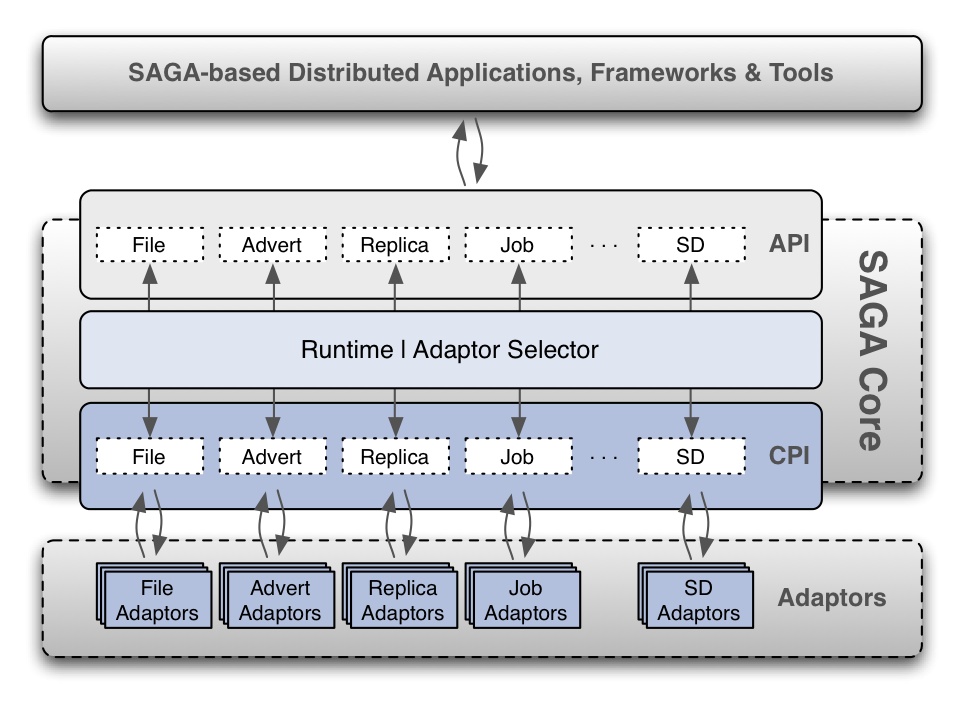
\includegraphics[width=0.66\textwidth]{figures/saga-architecture-1.png}
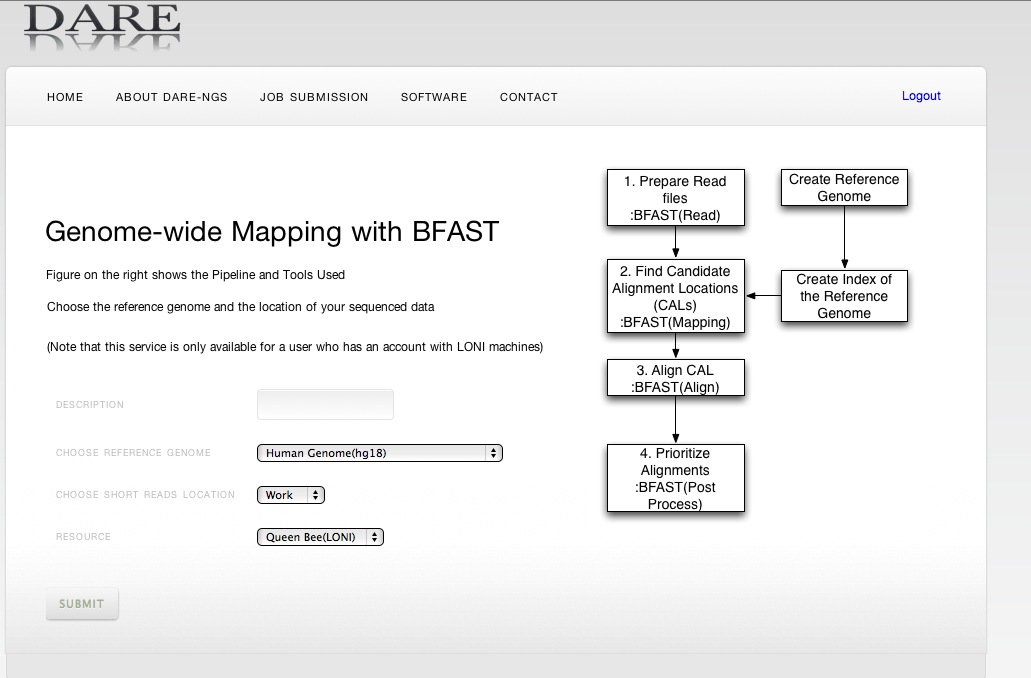
\includegraphics[width=0.5\textwidth]{figures/screenshot-ngs.png} \hspace{0.1in}
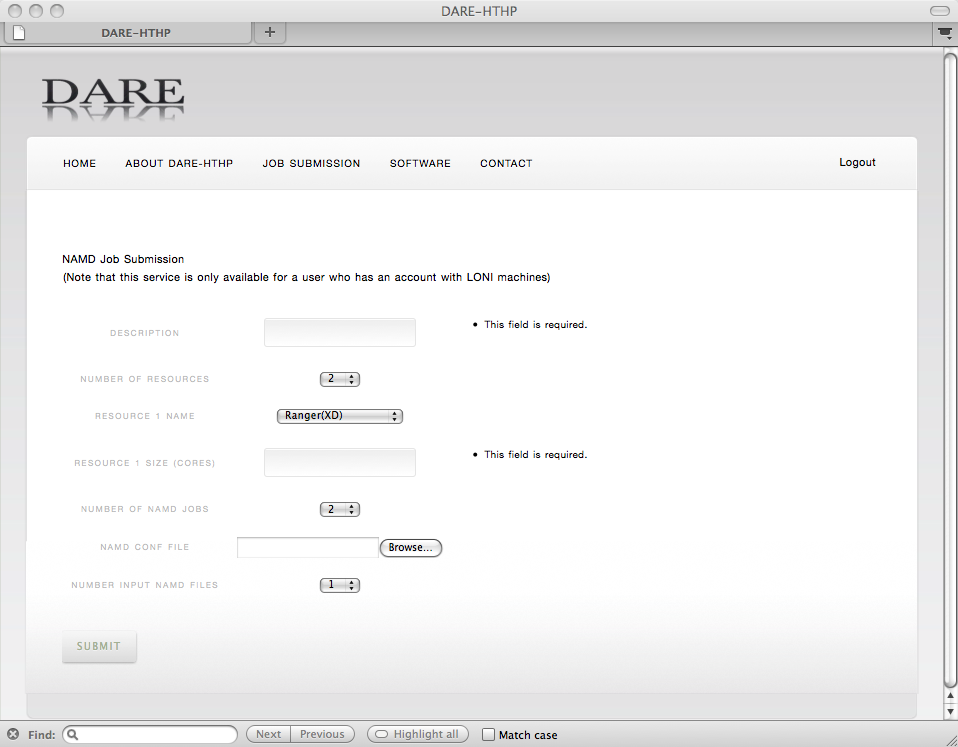
\includegraphics[width=0.42\textwidth]{figures/screenshot-hthp.png}
% }
\caption{\small (L) The User Interface of the DARE-NGS Gateway that
  utilizes DARE to execute BFAST (NGS) analytics. (R) NAMD job
  submission web page form through DARE-HTHP. Here, the form indicates
  the usage mode with multiple resources. The simple case with a
  single resource is default, and a user can expands the form by
  adding more resources as shown. DARE-HTHP and DARE-NGS can be
  accessed at: \url{http://dare.cct.lsu.edu} }
  \label{fig:NAMD2}
\end{figure}
\yyenote{The NAMD2 Figure is NOT referenced anywhere}

% \yyenote{Following sentence needs clarification} An important
% challenge in modern biomolecular simulations, that has received
% insufficient attention is to get single long-running jobs completed,
% but managing and executing multiple instances of the same (or
% similar) physical system. There are multiple reasons behind this --
% ranging from higher accuracy to reduced time-to-solution. For
% example, multiple ensemble-member runs of the same physical system
% enable better sampling In some cases, such as free-energy
% calculations, multiple ensembles of the same system need to be
% utilized. And even where a single long-running simulation is
% required, thanks to algorithmic advances, such problems can be
% transformed into the more {\it tractable} problem of solving
% multiple shorter run simulations.

\subsection{DARE-HTHP}

In addition to long time simulations of a single large system, an
important challenge is the ability to run a large number of identical
copies (ensembles) of the same system. Ensemble-based simulations are
important for effective sampling and due to the low-level of coupling
between them, ensemble-based simulations are good candidates to
utilize distributed cyberinfrastructure.  The problem for the
practitioner is thus effectively marshaling thousands if not millions
of high-performance simulations on distributed cyberinfrastructure.

Thus fundamental support for an ensemble of simulations with the
following characters is required: (i) Usable on a range of underlying
distributed resources and independent of resource-specific middleware
and services (i.e. scale-across), (ii) Efficiently manage both
scale-up and scale-out of ensembles -- possibly scaling up to
tens-of-thousands, if not millions of ensembles, with varying degrees
of coupling, (iii) Effective for a range of physical model sizes --
from thousands of atoms to hundreds of thousands of atoms, (iv) All of
the above without being tied to a specific underlying MD kernel, (v)
Extensible and Interoperable with emerging computational platforms
such as clouds.

It is important to establish that the challenges of supporting
ensemble-based MD simulations are different from traditional workflows
(e.g, SCEC~\cite{scec-sc10}), where the emphasis is on coordination of
pre-ordered tasks; by contrast ensemble-based simulations need to be
designed to support the optimal scale-out and scale-up of tasks across
multiple machines. In other words, in the latter, the makespan has to
be reduced by executing as many tasks concurrently as possible,
whereas in traditional workflows the makespan has to be reduced by the
efficient scheduling and placement of ordered tasks.

In Ref.~\cite{bigjob-ccgrid12} the ability of an {\it interoperable}
and {\it extensible} pilot-job tool (BigJob), to support
high-throughput simulations of high-performance molecular dynamics
simulations across distributed supercomputing infrastructure was
assessed.  Specifically, a nucleosome positioning problem as an
exemplar was used, wherein we computed 336 independent trajectories of
20 ns each.  Each trajectory was further divided into twenty 1 ns long
simulation tasks. A single task required $\approx$ 42~MB of input, 9
hours of compute time on 32 cores, and generated 3.8~GB of data.  In
total 6,720 tasks (6.7 $ \mu $s ) and approximately 25~TB were
managed.  There is natural task-level concurrency, as these 6,720 can
be executed with 336-way task concurrency.  A scalable pilot-job
approach was used to successfully complete this workload on the
TeraGrid/XSEDE.

% Using NAMD 2.7, this project
% requires approximately 2 million hours of CPU time and could be
% completed in just over 1 month on a dedicated supercomputer containing
% 3,000 cores.  In practice even such a {\it modest} supercomputer is a
% shared resource and our experience suggests that a simple scheme to
% automatically batch queue the tasks, might require several years to
% complete the project.

Building upon these results, DARE-HTHP provides an extensible
middleware wrapper around SAGA-BigJob, as evidenced by results
presented in Table~\ref{table:HTHP-Distributed} (from
Ref.~\cite{ccpe11}), which establish that that DARE-HTHP support
ensembles of simulations across a range of HPDC infrastructure.

% \jkimnote{need the attention for the following. one or two sentence
%   summary would be desirable}

%When the user submits the job to run on Futuregrid cloud environment
%the input files are transferred to different VM's. The configuration
%files that are prepared in the Access/Application layer will be used
%to launch the DARE Framework which in turn starts/submits according
%to the job configuration provided by user across Grids and Clouds.

% To provide the capability to run jobs in cloud using DARE, we have
% prepared images which have SAGA and other required adaptors installed
% along with NAMD and MPI as well. These images are used to launch
% multiple VM's and job submission similar to grid
% environment. Furthermore, we are in a process of proving a capability
% where a user can upload their images, and DARE will transfer them to
% Eucalyptus cloud on Futuregrid and run on virtualized environment; it
% is also responsible for marshaling the VM's and tasks in these
% environments.

 \begin{table}
\centering
\small
 \begin{tabular}{|c|c|c|c|c|c|c|} 
 \hline 
 Number           & Resource    & \# of &  \# of     &     \# of     &	TTC  \\
of tasks                &     &  Cores    &nodes&   VMs  & (sec) \\  
\hline
8& R&	64	&4 & - &141\\
\hline                  
8& QB	&	64& 8 &	-&176 \\
\hline
4/4&R/QB	&	32/32 &2/4&-&151\\
\hline
8&FG	&	64(8) & - &8&414 \\
\hline
2/3/3&R/QB/FG	&32/24/24&2/3&	3 &384\\
\hline


\end{tabular}
\caption{Time to completion (TTC) for 8 tasks of NAMD (each running on 8 cores,
  irrespective of the underlying resources), run over different resources. The three
  compute resources are Ranger (R), QueenBee (QB), 
  and  FutureGrid  Eucalyptus Cloud on Sierra(FG), respectively. The
  data shows that DARE-HTHC has been run successively on Grids and
  Clouds concurrently.}
 \label{table:HTHP-Distributed} 
\end{table}

\subsection{Other Examples}
\subsubsection{DARE-RFOLD}
\yyenote{The following is a re-write. Please check} 

We have developed DARE-RFOLD and successfully utilized for non-coding RNA
research and also to serve the RNA structure prediction
community. Through DARE-RFOLD, users can run simulations to predict
the Minimum Free Energy (MFE) secondary structure or to obtain an
ensemble of structures sampled with a Boltzmann-weighted sampling
scheme.

% To support nc-RNA research and broadly for the community who is
% interested in the utilization of RNA structure prediction for their
% research goals and education purposes, we have been developing a
% gateway, DARE-RFOLD, with which a user is able to predict the Minimum
% Free Energy (MFE) secondary structure or an ensemble of structure
% sampled with a Boltzmann-weighted sampling scheme.

Notably, our investigation into the computational requirements of RNA
folding (or structure prediction) suggest that the support of high-throughput
computation for a large number of tasks on heterogeneous distributed
resources is beneficial for the exploration of RNA folding energy
landscape and structural characterization of SAM-I riboswitch
sequences. As shown in Refs.~\cite{dare-ecmls11,ccpe11}, we demonstrated the DARE
framework and its ability to support many tasks of over multiple
scales and resources by effectively completing a
total of 2910 tasks needed for all known SAM-I RNA sequence family.

\subsubsection{DARE-DOCK}
DARE-DOCK aims the basic virtual screening.  The current
service with the gateway supports the docking with a popular
application, Autodock\cite{autodock}. \yyenote{The following sentence
  is five sentences rolled into one. Needs work}\jkimnote{i changed}
Specifically, the docking calculation is carried out with the recently
announced Autodock-vina, which allows to utilize fine-grain
parallelism with multi-threading multi-core support.  By supporting a service to run Autodock-vina, the gateway is able to carry out a
very effective execution of high-throughput docking with multiple
resources that is straightforwardly supported by DARE.

%\begin{figure}
% \centering
%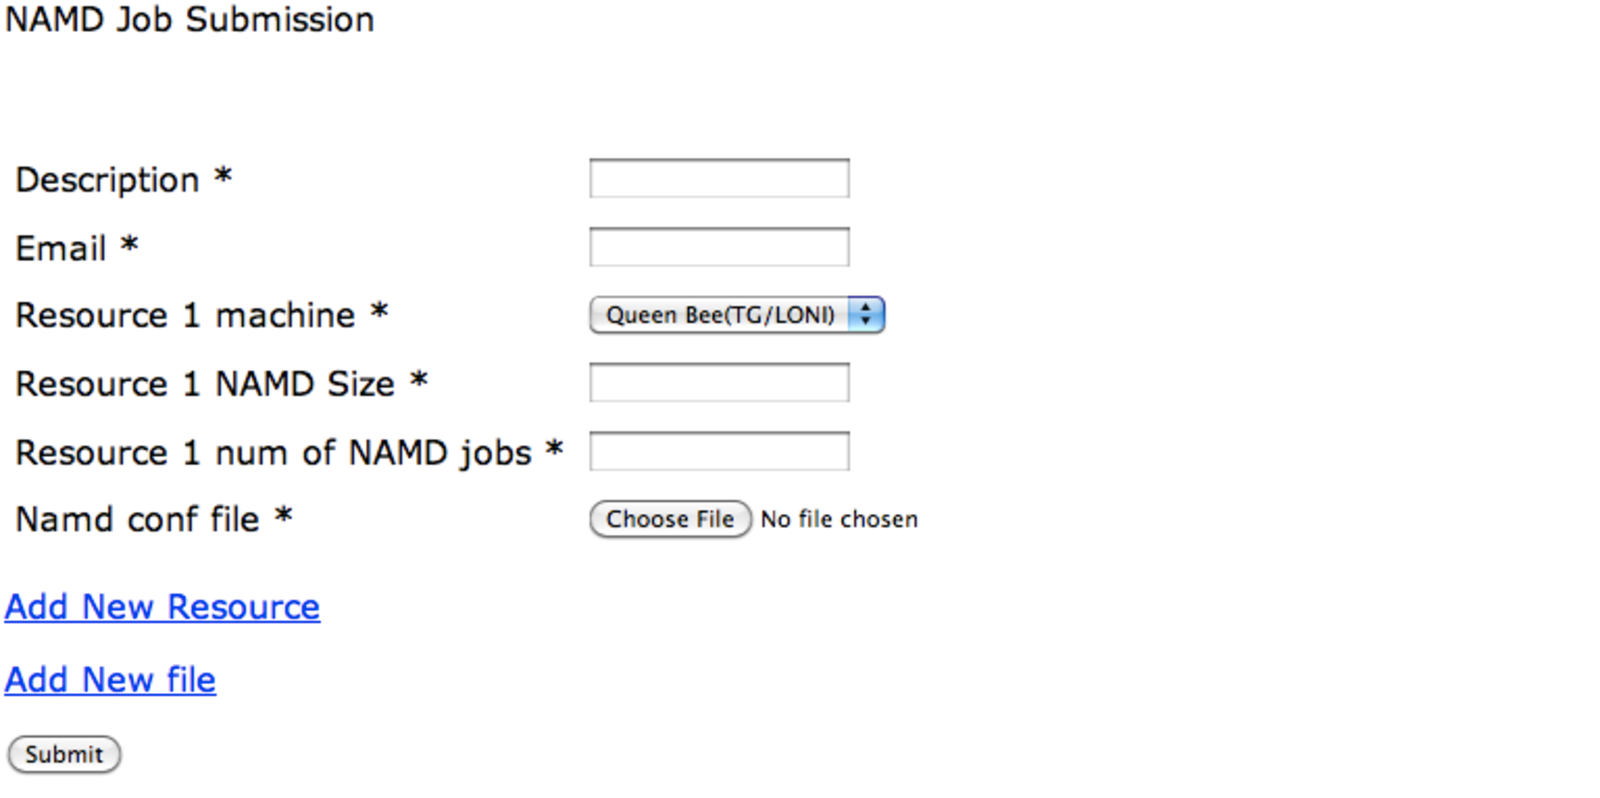
\includegraphics[scale=0.35]{figures/NAMD1.pdf}
%
%\caption{\small NAMD job submission web page form through DARE-HTHP} 
%\end{figure}

\section{Deploying DARE-based Gateways on TG/XSEDE}

There are two ways in which DARE-based Gateways can be provided to
users on XSEDE. The first involve the deployment of DARE-based
Gateways on a ``static'' resource -- with fixed connectivity, number
of users etc. The other involves the use of virtualized infrastructure
to support the deployment of ...

\subsection{Deploying DARE-based Gateways Using Virtualized Resource}
Indiana's Quarry~\cite{quarry} has been used as a novel agile virtual hosting
service for DARE-based gateways. Quarry is a gateway hosting resource
consisting of
geographically distributed Dell AMD systems that provide persistent,
secure virtualization services. Typically gateways would run
statically on dedicated hardware that is not directly connected (or
affiliated) with XSEDE systems. With Quarry, gateways can be run from
gateway-developer run images hosted on an XSEDE resource with high
bandwidth connections to XSEDE HPC resources as well as data
repositories at TACC (Ranch), NCSA (Forge) and PSC (Albedo).

There are many advantages to agile virtualized gateway systems
including automatic nightly backups, quick restores (if re-deploying
after failure), reduced maintenance and so on. Furthermore, the
virtualized solution has low operational costs, high bandwidth and
excellent support. There is however a unique advantage to gateway
framework developers: the ability to bundle a VM image containing the
gateway framework for immediate, user-ready deployment.  For DARE, the
bundled image will contain the basic framework along with
demonstration web interfaces: DARE-NGS and DARE-HTHP. If a third party
user (or gateway developer) wants to use DARE, all users have to do is
run the DARE image on Quarry and setup their credentials.

By contrast, most XSEDE (and formerly TeraGrid) science gateways ran
statically on hardware with low fault tolerance and custom web and
machine interfaces~\cite{xsedegateways}. In a
sense, this is a one-off custom solution that every group needing a
science gateway had to struggle with. Each of these gateways is a
unique installation running on user side resources with custom scripts
and more importantly custom interfaces to TeraGrid/XSEDE.  This
complicates the deployment and utilization model of science gateways:
each gateway has to be a full ground-up development project and the
entire development and deployment burden is placed on the gateway
developers.

The deployment and utilization model for DARE shifts the development
and deployment effort so that regular users (not necessarily gateway
developers) can get a basic science gateway running in quick order
without much difficulty.  With a basic understanding of gateways, a
user can start their own DARE VM on Quarry and customize the existing
building blocks and interfaces to their satisfaction. This reduces
XSEDE integration overhead, gateway development and deployment
overhead and unifies gateway infrastructure for many applications. It
is also important to note that other XSEDE sites are in the process of
deploying gateway hosting services similar to Quarry, and with VM
portability, DARE VM's can be ubiquitous on these resources as
well. Our expectation is to see science gateways as a generic but
customizable service available to users, complete with building blocks
in the form of ``canned'' virtual machine images.


\subsection{Data Management in DARE-based Gateways}
\yyenote{This paragraph needs revisiting}\jhanote{And moving..}

The two main features required for any science gateway are data
management and task management systems.  With the DARE framework, we
aim to provide a solution for many challenges associated with such
requirements, in particular in the context of the utilization of
distributed heterogeneous resources.  As mentioned earlier, the pilot
job abstraction, SAGA-BigJob, has been successfully developed for
distributed task management and integrated into the current DARE
framework as a key component.  For data management, SAGA-BigData is
being actively developed in parallel to BigJob.

The current implementation of DARE relies on data movement solutions
provided by SAGA, namely GridFTP and SCP. A Globus-Online adaptor is
being developed for SAGA, along with a DARE interface and a web
API. The concept is to provide web-users with an interface very
similar to Globus-Online, complete with scheduled file transfers,
third party transfers, pause/resume, bandwidth caps, error detection
and notification and routing options. A global file index is also
being developed to catalog input data sets and their locations, along
with locations of archived data around XSEDE resources. These DARE
capabilities provide data movement and orchestration necessary for
complex workflow support.

\section{Discussion}

% Conclusions} All of the components in the DARE-framework are
% independent of each other because to its modular design. The
% framework provides the key functionality of job and data management
% over heterogeneous distributed resources. This is provided so as to
% support various execution patterns and application usage modes as
% well as the full-functional access layer.

The fact that DARE has been used to support four very different
science applications is testimony to the correct abstractions and
design objectives.  In each case, DARE has facilitated the quick,
effective and scalable integration of the scientific logic associated
with the of a use-case/usage-mode (often implemented with python
scripts) with the underlying HPDC infrastructure/resources.  Each of
these science applications and their usage-modes have been supported
via both {\it command-line} as well as {\it science gateway}
interfaces.

% scalability ({\it distributed scale-out}) It is noticeable that we
% compare different usage modes, for example, using one resource or
% two resource altogether with the same configuration for the
% computation.

DARE supports the primary distributed application design objectives in
IDEAS~\cite{ideas} -- Interoperability, Dynamic execution,
Extensibility, Adaptivity and Scalability. One of these objectives,
scalability (in particular, scale-across), represents the ability to
utilize multiple resources; using these resources collectively has
many benefits, not least of which is the decrease in the
time-to-completion.  As illustrated in
Table~\ref{table:NGS-Distributed}, DARE has been used to demonstrate
such performance improvements; specifically, where two large TG/XSEDE
systems -- QB and Ranger, were used for the match step in BFAST
pipeline. For the HTHP mode~\cite{bigjob-ccgrid12}, upto 24,192 cores
were utilized at the same time, 128 concurrent simulations were
managed (scale-out) and upto four different TeraGrid/XSEDE resources
used. Given the difference in middleware distributions, this also
demonstrates DARE's ability to support interoperability.

% We have also used DARE-based gateways for
% efficient scale-out of multiple MD simulations in different usage
% modes.

% Not only have we
% established efficient distributed scale-out for data-intensive
% applications, we have shown the effective distribution of multiple MD
% simulations-- both in loosely-coupled and uncoupled ensemble-MD
% modes.

% While SAGA via the adaptor mechanism, provides the capabilities to
% expand the infrastructure it can be utilized on, e.g., t 

% Simple and effective extensibility is an important objective for
% gateways; indeed, many levels of extensibility are provided by
% DARE-based gateways. 

Functional and infrastructural extensibility are important
requirements for gateways; indeed, as we have shown, many levels of
extensibility are provided by DARE-based gateways.  For example, the
SAGA-based approach which provide numerous adaptors to different
middleware, supports interoperability across different middleware
types; it is limited only by the availability of adaptors (SAGA has
relevant adaptors to multiple existing infrastructure including
clouds).  The integration between L2 and L3 via different types of
services supported via a range of execution patterns and SAGA-based
pilot-abstractions, provide the flexibility to extend scientific
capability of a gateway, e.g., support of ensemble-based simulations
as a primitive ``execution unit''.  Building upon the
Pilot-abstractions, DARE-based gateways also support extended
data-access patterns and coupled data-compute placement.  Functional
extensibility is required for scientific inquiry; for example, with
DARE-RFOLD, we have provided a pipeline whereby the output from the
RNA secondary structure prediction was utilized for Riboswitch gene
annotation using structural information.


% for another capability beyond RNA secondary structure prediction. We
% demonstrated recently that Furthermore, with the open source pylons
% framework, incorporation of web technologies is efficiently and
% easily achieved.

% Note that not only varying the size of a BigJob, other possible usage
% modes supporting a case of loosely coupled applications~\cite{coupled}
% and a case of dynamically changing parallel/concurrent configurations
% in the fine-grain parallelization (for example, MPI configuration) as
% well as the coarse-grain parallelization are effectively designed.

The experience of using DARE to support NGS analytics over a range of
input problem sizes, infrastructure and analytical problems, (as
illustrated by Table~\ref{table:NGS-Distributed}), indicate that
Science-Gateways for distributed data-intensive applications have a
set of unique challenges. For example, for NGS data alignment using
BFAST, not only does one need to determine the right distribution of
computational resources for the given tasks/problem at hand, but these
tasks need to be placed ``optimally'' so that data movement does not
become the bottleneck. DARE supports such {\it dynamic} resource
utilization and execution capabilities.

% distributed abilities, optimal task-level concurrency based upon how
% the reference genome indexes are utilized for chunks of short read
% data\cite{dare-ecmls11} are required; for example, or

In conjunction with the ability to distribute tasks effectively, NGS
data alignment using BFAST, requires the ability to determine the
optimal task-level concurrency; this is often a function of how the
reference genome indexes are utilized for chunks of short read
data\cite{dare-ecmls11}.  The design of the DARE framework supports
such application-level adaptivity, via support for flexible
composition of L2 services, and flexible execution patterns and
dynamic execution modes. As alluded to in \S~2.1, application-level
requirements must be matched by the runtime systems; here the runtime
systems such as SAGA-based pilot-jobs support application-level
adaptivity, e.g., change in task-level granularity, usage modes etc.
Other forms of adaptivity supported by the runtime systems that
DARE-based Gateways build upon, include different data-transfer
mechanisms -- varying from gridFTP, to reliable protocols and variants
thereof (such as GlobusOnline).

% in conjunction with distributed abilities, these tasks need to be
% placed ``optimally'' so that data movement does not become the
% bottleneck. DARE supports such {\it dynamic} resource utilization and
% execution capabilties.

It is important to reiterate, that all of the objectives as captured
by IDEAS are provided by DARE using distributed computing community
{\it standards}. The lack of need to change interfaces and development
systems imparts a simplicity to the development process, i.e., SAGA is
the basis for the simplicity ensuing from the well defined interfaces
that supports multiple {\it standards} distributed functionality, as
well as higher-level abstractions, e.g., based on the underlying
SAGA-based API, via SAGA-BigJob a general purpose Pilot-Job
abstraction.

Finally, the new virtual machine image based deployment model on
Indiana's Data Quarry system enables rapid and hassle free
deployment. No hardware needs to be purchased, no backups arranged,
and web development. In due time, we expect to have popular content
management systems with DARE infrastructure available in images for
the entire community to use.

In summary, we have demonstrated via working examples, how providing
the right abstractions and easy integration with other components,
enables DARE-based gateways to support the effective and easy
development of science gateways for life-science applications that
support distributed applications, whilst adhering to the IDEAS
design-objectives. This includes advanced deployment modes and novel
data-intensive life-science applications that utilize emerging
distributed computing/data resources such as TG/XSEDE and cloud
environment contributes.

\section*{Acknowledgments}
This work is primarily supported and motivated by Grant Number
P20RR016456 from the NIH National Center For Research Resources. We
are grateful to Andre Luckow and Ole Weidner for their work for SAGA
and SAGA-BigJob development; we also thank Ole Weidner for a
constructive criticism of this manuscript and Andre Merzky for the information about SAGA CSA deployment. Computing resources used for this work were made possible via NSF TRAC award TG-MCB090174 and
LONI resources. This document was developed with support from the
National Science Foundation (NSF) under Grant No. 0910812 to Indiana
University for ``FutureGrid: An Experimental, High-Performance Grid
Test-bed.''. SJ would like to thank Dave Hart (SDSC) and Dan Katz
(Chicago) for helpful discussions.


%\bibliographystyle{spbasic}      % basic style, author-year citations
%\bibliographystyle{spmpsci}      % mathematics and physical sciences
%\bibliographystyle{spphys}       % APS-like style for physics

%\bibliographystyle{abbrv}
\bibliographystyle{unsrt}
%\bibliography{saga,tg11}
\bibliography{saga,jogc}
\end{document}

